% ============================================================
%  Causal Machine Unlearning via Counterfactual World Modeling
%  NeurIPS 2025 Format
%
%  Compile:  pdflatex paper.tex && bibtex paper && pdflatex paper.tex && pdflatex paper.tex
%  Figures:  python generate_figures.py   (from paper/ directory)
% ============================================================

\documentclass{article}
\usepackage[preprint]{neurips_2026}   % swap to [final] for camera-ready

% ── Core packages ──────────────────────────────────────────────────────────
\usepackage[utf8]{inputenc}
\usepackage[T1]{fontenc}
\usepackage{hyperref}
\usepackage{url}
\usepackage{microtype}
\usepackage{xcolor}

% ── Math ───────────────────────────────────────────────────────────────────
\usepackage{amsmath,amssymb,amsthm}
\newtheorem{proposition}{Proposition}
\usepackage{nicefrac}
\usepackage{bbm}

% ── Tables \& Figures ──────────────────────────────────────────────────────
\usepackage{booktabs}
\usepackage{multirow}
\usepackage{graphicx}
\usepackage{subcaption}
\usepackage{enumitem}

% ── TikZ (concept diagram) ─────────────────────────────────────────────────
\usepackage{tikz}
\usetikzlibrary{arrows.meta, positioning, shapes.geometric,
                calc, fit, backgrounds, decorations.pathreplacing}

% ── Algorithm ──────────────────────────────────────────────────────────────
\usepackage{algorithm}
\usepackage{algpseudocode}

% ── Custom macros ──────────────────────────────────────────────────────────
\newcommand{\doop}{\mathrm{do}}
\newcommand{\CE}{\mathrm{CE}}
\newcommand{\Dfid}{\mathcal{D}_{\mathrm{fid}}}
\newcommand{\Loss}{\mathcal{L}}
\newcommand{\Pw}{P_w}
\newcommand{\Pwt}{P_{w^\tau}}
\newcommand{\ptheta}{p_{\theta}}
\newcommand{\RR}{\mathbb{R}}
\newcommand{\EE}{\mathbb{E}}

% ── Colors ─────────────────────────────────────────────────────────────────
\definecolor{myred}{RGB}{192,57,43}
\definecolor{mygreen}{RGB}{39,174,96}
\definecolor{myblue}{RGB}{41,128,185}
\definecolor{mygray}{RGB}{127,140,141}

% ===========================================================================
\title{Causal Machine Unlearning via Counterfactual World Modeling}
% ===========================================================================

\author{
  Kseniia Kuvshinova \\
  Machine Learning Department \\
  Mohamed Bin Zayed University of AI \\
  \texttt{kseniia.kuvshinova@mbzuai.ac.ae} \\
  \And
  Mohammed Talha Alam \\
  Machine Learning Department \\
  Mohamed Bin Zayed University of AI \\
  \texttt{mohammed.alam@mbzuai.ac.ae}
}

\begin{document}
\maketitle

% ===========================================================================
\begin{abstract}
% ===========================================================================
We study \emph{post-hoc concept-level unlearning}: producing, from a
spuriously-trained model, a behavioural approximation of what the model would
have been if a designated concept had been causally decoupled from the label.
We formalise this as a do-calculus intervention on the training SCM and prove
that minimising the population paired-counterfactual KL drives counterfactual
output invariance.  The resulting algorithm fine-tunes the pre-trained model
with a 3-term loss: cross-entropy $+\lambda\!\cdot\!\CE_C(\theta) + \beta$-locality.
On Colored MNIST (3 seeds) the CE penalty achieves a normalised
$86.9 \pm 2.7\%$ reduction in CE---the most cross-seed-stable headline number
in the paper---while preserving 87\%+ observational accuracy.
On Waterbirds (3 seeds, ResNet-18) our method, using only paired
counterfactuals, achieves the best average accuracy ($85.2\%$) and best CE
reduction ($1.56\!\to\!0.97$, $-38\%$) among single-environment post-hoc
baselines; group-balanced DFR \cite{kirichenko2023last} attains the highest
worst-group accuracy ($87.3\%$).  On CelebA blond/gender (3 seeds, ResNet-50,
20k train subset; absolute numbers not directly comparable to full-CelebA
literature) $\lambda{=}0.1$ delivers a \emph{statistically supported}
worst-group gain of $+12.4$~pp [$+6.5, +17.9$] over the no-unlearning
baseline (closing 83\% of the oracle gap), with the lowest mean $\CE_C$
(at $\lambda{=}1.0$, $0.16 \pm 0.04$) and lowest mean distance to oracle
($0.08 \pm 0.01$) of all post-hoc methods.  We are explicit about the
operating-point trade-off: at higher $\lambda$ on CelebA, the same setting
that minimises $\CE_C$ also \emph{worsens} worst-group accuracy below
baseline---an honest failure mode of the surrogate under extreme class
imbalance, discussed in detail in \S\ref{subsec:celeba} and Limitation 7.
We also characterise robustness to limited (5\%), noisy ($\sigma\!\le\!0.1$),
and approximate counterfactual supervision; show via linear probing that our
method achieves the \emph{same output-level} forgetting regime as the
oracle (concept remains decodable from features in both); and plot the joint
CE / distance-to-oracle Pareto frontier.
\end{abstract}

% ===========================================================================
\section{Introduction}
\label{sec:intro}
% ===========================================================================

A growing literature on \emph{machine
unlearning}~\cite{cao2015machine,guo2020certified,gupta2021adaptive,sekhari2021remember,bourtoule2021machine}
seeks to modify a trained model so that it behaves as if a specified subset of training
data had never been seen.  Most existing work formalises this at the \emph{sample
level}, targeting individual training examples or small forget sets and measuring
success by statistical indistinguishability from a model retrained without those
examples.  Such methods are the appropriate tool when the goal is a privacy
\emph{certificate} for an individual record (e.g.\ enforcing a GDPR-style
deletion request).

This sample-level view is insufficient for a broad and practically important
class of unlearning requests: \emph{concept-level} forgetting.  Consider a
model trained on Colored MNIST, where digits 0--4 are predominantly red and
5--9 predominantly green with 90\% probability.  The model rapidly learns
colour as a near-optimal proxy for the digit label.  A request to ``forget
colour'' cannot be satisfied by removing a few samples: the spurious
correlation is distributed throughout the entire training set.  What the
practitioner needs is a model that behaves \emph{as if it had been trained
in a world where colour and label were independent}---a fundamentally causal
statement.  We treat this as a \emph{behavioural approximation} problem:
producing a model whose predictive distribution matches the intervened-world
oracle.  This is distinct from---and complementary to---the certificate-style
sample-level objective; we discuss the relationship explicitly in
\S\ref{sec:discussion}.

\textbf{This paper proposes a causal view of machine unlearning.}  We model the
training distribution as arising from a structural causal model (SCM)
$\mathcal{M}$ with variables $(X, C, Y)$: $X$ is core content (digit shape),
$C$ is the spurious concept (color), and $Y$ is the target label.  An unlearning
request for $C$ is formalized as the causal intervention
$\doop(C{\sim}\mathrm{Bern}(\nicefrac{1}{2}))$, which severs the dependence of
$C$ on $Y$ and yields a counterfactual world $w^\tau$.  The oracle target
$\theta^*$ is the model retrained from scratch on $w^\tau$.  Unlike sample
removal, this intervention unambiguously specifies \emph{what to forget} (the
causal pathway from $C$ to predictions) and \emph{how to measure success}
(distributional fidelity to $\theta^*$ and counterfactual invariance of
predictions under interventions on $C$).

We make the following \textbf{contributions}:
\begin{enumerate}[leftmargin=1.5em]
  \item \textbf{Causal framework and surrogate.}  We frame post-hoc
    concept-level unlearning as approximation to an intervened-world oracle
    via a do-calculus operation on the training SCM, define a tractable
    paired-counterfactual surrogate $\CE_C(\theta)$, and prove that
    $\CE_C(\theta){=}0$ implies counterfactual output invariance under the
    estimator's measurability assumptions (\S\ref{sec:framework},\,\S\ref{sec:method}).
  \item \textbf{Composite post-hoc algorithm with broad validation.}  We
    propose a 3-term loss (retain $+ \lambda\cdot\CE_C + \beta$-locality) and
    evaluate it across two benchmarks (Colored MNIST and Waterbirds), three
    seeds, and seven baselines (naive FT, IFT, GRL, concept erasure via
    linear projection, oracle distillation, plus our $\lambda$-sweep), with
    consistent multi-seed reporting (\S\ref{sec:experiments}).
  \item \textbf{Practicality analysis.}  We characterize the method under
    \emph{realistic supervision}: data efficiency (5--100\% of pairs),
    noisy counterfactuals ($\sigma{\in}[0,0.5]$), approximate
    counterfactuals (Waterbirds: same-class different-background), output- vs.\
    representation-level forgetting via linear probing, and the joint
    CE/distance-to-oracle frontier (\S\ref{sec:experiments}).
\end{enumerate}

% ===========================================================================
\section{Related Work}
\label{sec:related}
% ===========================================================================

\paragraph{Machine unlearning.}
The machine unlearning problem was first formalized by~\citet{cao2015machine};
\citet{bourtoule2021machine} proposed exact unlearning via data partitioning
(SISA).  Approximate methods include influence-function-based certified data
removal~\cite{guo2020certified} and Newton-step
updates~\cite{sekhari2021remember}.  \citet{gupta2021adaptive} studied adaptive
adversaries.  All these works target \emph{sample-level} forgetting.  Our work
targets \emph{concept-level} forgetting, where the forget set is a statistical
dependence encoded across the full training distribution, not a finite collection
of examples.

\paragraph{Spurious correlations and invariant learning.}
Invariant Risk Minimization~\cite{arjovsky2019irm} and group Distributionally
Robust Optimization~\cite{sagawa2020dro} train models that are invariant to
environment-specific spurious correlations.  These require multi-environment
or group-labelled data \emph{at training time}.  Without group labels at
training, related approaches reweight or re-train selectively: \emph{Just
Train Twice}~\cite{liu2021jtt} upweights examples misclassified by an ERM
model, \emph{Learning from Failure}~\cite{nam2020lff} uses a biased classifier
to identify minority samples, and \emph{Deep Feature
Reweighting}~\cite{kirichenko2023last} retrains only the last linear layer on
a small group-balanced reweighting set—an especially relevant baseline that
we compare to in \S\ref{subsec:waterbirds}.

\paragraph{Causal approaches to spurious correlation.}
\citet{veitch2021counterfactual} formalise counterfactual invariance for text
classifiers under a stable / spurious decomposition; their target object
(invariance to do-interventions on a covariate) is the same family as our
$\CE_C(\theta)$ but they study training-time augmentation rather than
post-hoc fine-tuning.  \citet{makar2022causally} use auxiliary labels to
construct a causally motivated regulariser on training distributions.
Our contribution differs from these in three ways: (i) the model is
\emph{already trained} (post-hoc setting), (ii) the formal target is the
intervened-world oracle's output distribution rather than environment
invariance, and (iii) we evaluate against a stricter baseline matrix that
explicitly distinguishes group-supervised from single-environment methods.
Recent work on concept erasure in language model
representations~\cite{belrose2023concept} removes linear projections of
concept directions; we directly penalise causal influence on the output
distribution and characterise empirically that this is the regime the oracle
itself occupies (\S\ref{subsec:probing}).

\paragraph{Adversarial debiasing.}
Domain-adversarial training~\cite{ganin2016domain} uses a gradient reversal
layer (GRL) to make learned features unable to predict a nuisance attribute.
This is typically applied \emph{at training time} with multi-task learning;
applying it post-hoc (fine-tuning with gradient reversal) is a natural baseline.
We empirically show that post-hoc GRL is unstable and degrades significantly
below the original baseline, whereas our approach is stable and improves
over baseline on all metrics (\S\ref{sec:experiments}).

\paragraph{Counterfactual fairness and causal ML.}
\citet{kusner2017counterfactual} define individual fairness via counterfactual
invariance: a prediction is fair if it does not change when a sensitive
attribute is intervened upon.  Our CE proxy $\CE_C(\theta)$ is directly
inspired by this notion and operationalizes it as a post-hoc training signal.
Pearl's do-calculus~\cite{pearl2009causality} provides the theoretical
foundation for our intervention-based world model.
\citet{scholkopf2021causal} survey causal representation learning more broadly;
our work is a post-hoc version.

\paragraph{Knowledge editing.}
ROME~\cite{meng2022rome} and MEMIT~\cite{meng2022memit} surgically modify
factual associations in LLMs.  These target declarative knowledge rather than
statistical dependences from spurious correlations, and differ structurally
from our setting.

% ===========================================================================
\section{Causal Framework for Machine Unlearning}
\label{sec:framework}
% ===========================================================================

\subsection{Structural Causal Model and Observational World}

We model the data-generating process as an SCM
$\mathcal{M} = (\mathbf{V}, \mathbf{E}, \mathbf{F}, P_\mathbf{N})$ over
observed variables $\mathbf{V} = \{X, C, Y\}$:
\begin{itemize}[leftmargin=1.5em]
  \item $Y \in \{0, \ldots, 9\}$: the target label (digit identity).
  \item $X \in \RR^{3 \times H \times W}$: the core content (digit image colored by $C$).
  \item $C \in \{0, 1\}$: the spurious concept/attribute (color: red or green).
\end{itemize}
In the \emph{observational world} $w$, the structural equations generate a
strong spurious association: digits $0$--$4$ receive $C=0$ (red) and digits
$5$--$9$ receive $C=1$ (green) with probability $\rho = 0.9$:
$C \mid Y \sim \mathrm{Bern}(\rho \cdot \mathbbm{1}[Y \geq 5]
+ (1{-}\rho) \cdot \mathbbm{1}[Y < 5])$.
The joint training distribution is $\Pw(X, C, Y)$.

\subsection{Intervention-Defined Unlearning}

An unlearning request for concept $C$ asks: \emph{produce a model that behaves
as if $C$ were causally uninformative about $Y$}.  We formalize this as a
causal intervention:
\begin{equation}
  w^\tau = \doop_\tau(w), \qquad \tau: C \sim \mathrm{Bern}\!\left(\nicefrac{1}{2}\right).
  \label{eq:intervention}
\end{equation}
This surgically modifies the structural equation for $C$—replacing it with an
independent draw—while leaving all other equations intact.  The resulting
$\Pwt(X, C, Y)$ satisfies $C \perp Y$.  Figure~\ref{fig:concept} illustrates the
two worlds.

\subsection{Oracle Target and Evaluation Criteria}

Let $\theta_0$ be a model trained on $\Pw$.  The
\emph{oracle retrained} model $\theta^*$ is trained from scratch on $\Pwt$;
it is the ground-truth target any post-hoc algorithm should approximate.

We adopt three evaluation criteria:

\textbf{(1) Retained utility.}
\begin{equation}
  \mathcal{U}(\theta^-) = \EE_{(x,c,y) \sim \Pw}\!\left[\mathbbm{1}[\arg\max \ptheta^-(y' \mid x, c) = y]\right].
\end{equation}

\textbf{(2) Causal forgetting.}  Predictions should be invariant to
interventions on $C$ holding $X$ fixed.  We measure this via the
\emph{causal effect proxy}:
\begin{equation}
  \CE_C(\theta) = \EE_{x \sim \Pwt(X)}\,\EE_{c_0, c_1 \sim \Pwt(C)}
  \!\left[\mathrm{KL}\!\left(\ptheta(\cdot \mid x, c_0)\,\big\|\,\ptheta(\cdot \mid x, c_1)\right)\right].
  \label{eq:ce}
\end{equation}
$\CE_C(\theta^*) \approx 0$ is the gold standard; $\CE_C(\theta_0) \gg 0$
reflects the spurious dependence.

\textbf{(3) Fidelity to retraining.}
\begin{equation}
  \Dfid(\theta^-, \theta^*) = \EE_{(x,c) \sim \Pwt}\!\left[
    \mathrm{KL}\!\left(\ptheta^-(\cdot \mid x, c)\,\big\|\,\ptheta^*(\cdot \mid x, c)\right)
  \right].
  \label{eq:fidelity}
\end{equation}

% ── Figure 1: Concept Diagram ──────────────────────────────────────────────
\begin{figure*}[t]
\centering
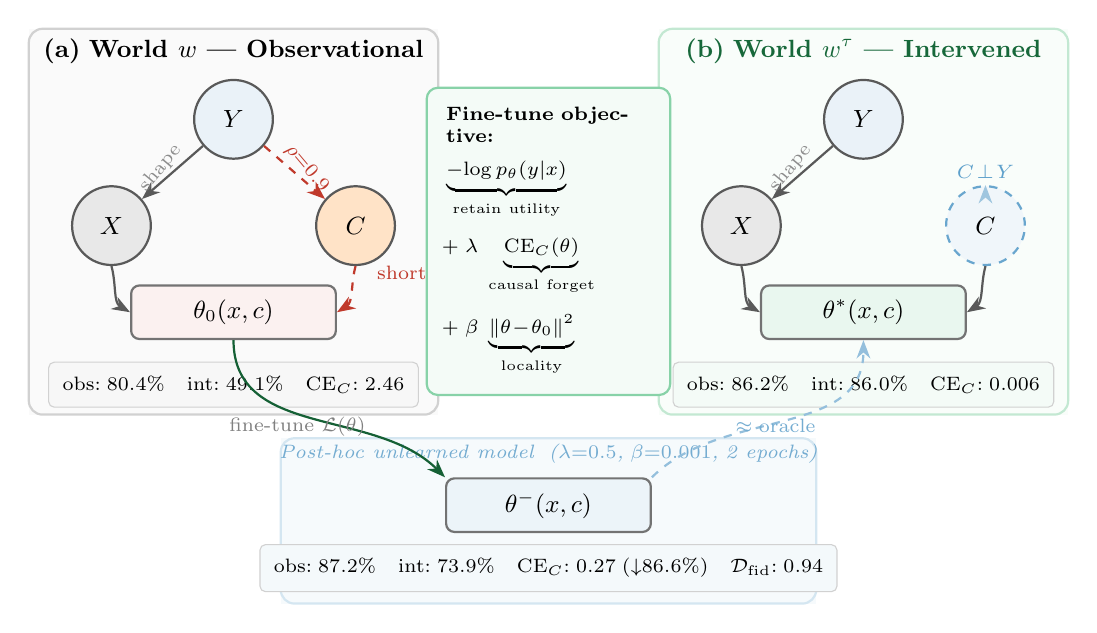
\begin{tikzpicture}[
  cn/.style={circle, draw=black!65, thick, minimum size=10mm,
             font=\small, inner sep=0pt},
  iv/.style={circle, draw=myblue!70, thick, dashed, minimum size=10mm,
             font=\small, inner sep=0pt, fill=myblue!7},
  mb/.style={rectangle, draw=black!55, thick, rounded corners=3pt,
             minimum width=2.6cm, minimum height=0.68cm,
             font=\small, align=center},
  sb/.style={rectangle, draw=black!18, rounded corners=2pt,
             fill=gray!6, font=\scriptsize, inner sep=5pt, align=left},
  ea/.style={-Stealth, thick, black!65},
  es/.style={-Stealth, thick, dashed, myred},
]

% ══════════════════════════════════════════════════════════════════════════
% BACKGROUND PANELS
% ══════════════════════════════════════════════════════════════════════════
\fill[gray!4]     (0.00, 2.30) rectangle (5.20, 7.20);
\draw[black!18, thick, rounded corners=5pt]
  (0.00, 2.30) rectangle (5.20, 7.20);

\fill[mygreen!3]  (8.00, 2.30) rectangle (13.20, 7.20);
\draw[mygreen!28, thick, rounded corners=5pt]
  (8.00, 2.30) rectangle (13.20, 7.20);

% UNLEARNED MODEL STRIP
\fill[myblue!4]   (3.20, -0.10) rectangle (10.00, 2.00);
\draw[myblue!20, thick, rounded corners=5pt]
  (3.20, -0.10) rectangle (10.00, 2.00);

% ══════════════════════════════════════════════════════════════════════════
% PANEL A — World w  (Observational)
% ══════════════════════════════════════════════════════════════════════════
\node[font=\small\bfseries] at (2.60, 6.92)
  {(a)\;World $w$ — Observational};

\node[cn, fill=myblue!10] (Y1) at (2.60, 6.05) {$Y$};
\node[cn, fill=gray!18]   (X1) at (1.05, 4.70) {$X$};
\node[cn, fill=orange!22] (C1) at (4.15, 4.70) {$C$};

\draw[ea] (Y1) -- (X1);
\node[font=\scriptsize, black!45, rotate=50]  at (1.67, 5.43) {shape};
\draw[es] (Y1) -- (C1);
\node[font=\scriptsize, myred,    rotate=-50] at (3.53, 5.43) {$\rho{=}0.9$};

\node[mb, fill=myred!7] (m0) at (2.60, 3.60) {$\theta_0(x,c)$};
\draw[ea] (X1.south) to[out=285, in=150] (m0.west);
\draw[es] (C1.south) to[out=255, in=32]  (m0.east);
\node[font=\scriptsize, myred, anchor=west] at (4.30, 4.10) {shortcut};

\node[sb] at (2.60, 2.68) {%
  obs:\;$80.4\%$\quad int:\;$49.1\%$\quad $\CE_C$:\;$2.46$};

% ══════════════════════════════════════════════════════════════════════════
% CENTRE — Intervention arrow + fine-tune objective
% ══════════════════════════════════════════════════════════════════════════
\draw[-Stealth, line width=1.8pt, myblue!80]
  (5.50, 5.90) -- (7.70, 5.90)
  node[midway, above, font=\small, myblue!80]
  {$\doop\!\bigl(C\sim\mathrm{Bern}(\nicefrac{1}{2})\bigr)$};

\node[draw=mygreen!55, thick, fill=mygreen!5, rounded corners=4pt,
      font=\scriptsize, inner sep=7pt, text width=2.6cm, align=left]
  (lb) at (6.60, 4.50)
  {\textbf{Fine-tune objective:}\\[4pt]
   $\underbrace{-\!\log p_\theta(y|x)}_{\text{retain utility}}$\\[6pt]
   $+\;\lambda\;\underbrace{\CE_C(\theta)}_{\text{causal forget}}$\\[6pt]
   $+\;\beta\;\underbrace{\|\theta\!-\!\theta_0\|^2}_{\text{locality}}$};

% ══════════════════════════════════════════════════════════════════════════
% PANEL B — World w^τ  (Intervened)
% ══════════════════════════════════════════════════════════════════════════
\node[font=\small\bfseries, mygreen!60!black] at (10.60, 6.92)
  {(b)\;World $w^\tau$ — Intervened};

\node[cn, fill=myblue!10] (Y2) at (10.60, 6.05) {$Y$};
\node[cn, fill=gray!18]   (X2) at  (9.05, 4.70) {$X$};
\node[iv]                  (C2) at (12.15, 4.70) {$C$};

\draw[ea] (Y2) -- (X2);
\node[font=\scriptsize, black!45, rotate=50] at (9.67, 5.43) {shape};

\node[font=\scriptsize, myblue!75, anchor=center] at (12.15, 5.38)
  {$C\!\perp\!Y$};
\draw[-Stealth, thick, myblue!45, dashed]
  (12.15, 5.16) -- (C2.north);

\node[mb, fill=mygreen!10] (ms) at (10.60, 3.60) {$\theta^*(x,c)$};
\draw[ea] (X2.south) to[out=285, in=150] (ms.west);
\draw[ea] (C2.south) to[out=255, in=32]  (ms.east);

\node[sb, fill=mygreen!5] at (10.60, 2.68) {%
  obs:\;$86.2\%$\quad int:\;$86.0\%$\quad $\CE_C$:\;$0.006$};

% ══════════════════════════════════════════════════════════════════════════
% BOTTOM STRIP — Unlearned model θ⁻
% ══════════════════════════════════════════════════════════════════════════
\node[font=\scriptsize\itshape, myblue!65] at (6.60, 1.80)
  {Post-hoc unlearned model \;($\lambda{=}0.5$,\;$\beta{=}0.001$,\;2 epochs)};

\node[mb, fill=myblue!9] (mu) at (6.60, 1.15) {$\theta^-(x,c)$};

\node[sb, fill=myblue!5] at (6.60, 0.35) {%
  obs:\;$87.2\%$\quad
  int:\;$73.9\%$\quad
  $\CE_C$:\;$0.27$\;(${\downarrow}86.6\%$)\quad
  $\Dfid$:\;$0.94$};

% ── Connecting arrows ──────────────────────────────────────────────────
\draw[-Stealth, thick, mygreen!55!black]
  (m0.south) to[out=270, in=135] (mu.north west);
\node[font=\scriptsize, black!50, anchor=east] at (4.40, 2.15)
  {fine-tune $\mathcal{L}(\theta)$};

\draw[-Stealth, thick, myblue!50, dashed]
  (mu.north east) to[out=45, in=270] (ms.south);
\node[font=\scriptsize, myblue!65, anchor=west] at (8.85, 2.15)
  {$\approx$\;oracle};

\end{tikzpicture}
\caption{%
  \textbf{Causal framework for concept-level machine unlearning.}
  \textbf{(a)} In world $w$, the training distribution carries a 90\% spurious
  correlation between color $C$ and label $Y$.  The baseline $\theta_0$
  exploits this shortcut (int-acc $49.1\%$, $\CE_C{=}2.46$).
  \textbf{Center:} The unlearning request is cast as
  $\doop(C{\sim}\mathrm{Bern}(\nicefrac{1}{2}))$.  We post-hoc fine-tune
  $\theta_0$ with a three-term composite loss.
  \textbf{(b)} In the counterfactual world $w^\tau$, $C\!\perp\!Y$; the oracle
  $\theta^*$ achieves near-zero causal effect ($\CE_C{=}0.006$).
  \textbf{Bottom:} Our unlearned model $\theta^-$ ($\lambda{=}0.5$, 2 epochs,
  averaged over 3 seeds) reduces $\CE_C$ by 86.6\% and gains $+19.1$~pp on
  intervened accuracy.
}
\label{fig:concept}
\end{figure*}


% ===========================================================================
\section{Method}
\label{sec:method}
% ===========================================================================

\subsection{Causal Effect Proxy via Paired Counterfactuals}

Equation~\eqref{eq:ce} defines $\CE_C(\theta)$ as the expected KL divergence
between model predictions under two different values of $C$ for the same content
$X$.  We estimate it using the paired counterfactual structure of our dataset.
For each training example $(x, c, y)$, we construct a counterfactual partner
$(x, c', y)$ with $c' = 1 - c$ (same digit image, opposite color).  The
per-sample contribution is:
\begin{equation}
  \widehat{\CE}_C(\theta;\, x, c) =
    \tfrac{1}{2}\left[
      \mathrm{KL}\!\left(\ptheta(\cdot \mid x, c)\;\big\|\;\ptheta(\cdot \mid x, c')\right)
      + \mathrm{KL}\!\left(\ptheta(\cdot \mid x, c')\;\big\|\;\ptheta(\cdot \mid x, c)\right)
    \right],
  \label{eq:ce_sym}
\end{equation}
the symmetric (Jensen--Shannon-like) KL.  This estimator requires no knowledge
of the SCM structure: any batch of (factual, counterfactual) pairs suffices.

\paragraph{Formal connection to counterfactual invariance.}
The surrogate $\CE_C$ is principled in the following sense.

\begin{proposition}[Population CE minimisation implies counterfactual invariance]
\label{prop:ce-invariance}
Let $\theta$ produce a strictly positive predictive distribution
$\ptheta(\cdot\mid x,c)$ on a finite output space, and let
$P_{w^\tau}(X, C, C')$ denote the joint distribution over content $X$ and
intervention pair $(C, C')$ in the counterfactual world $w^\tau$, with $C'$
denoting the counterfactual concept value.  Define
\[
  \CE_C(\theta) \;=\;
  \EE_{(X,C,C')\sim P_{w^\tau}}\!\bigl[\,\mathrm{KL}\bigl(\ptheta(\cdot\mid X, C)\,\big\|\,\ptheta(\cdot\mid X, C')\bigr)\bigr].
\]
Then $\CE_C(\theta) = 0$ if and only if
$\ptheta(\cdot\mid x, c) = \ptheta(\cdot\mid x, c')$ for $P_{w^\tau}$-almost every
$(x, c, c')$, i.e.\ $\theta$'s output distribution is invariant to interventions on $C$ holding $X$ fixed.
\end{proposition}

\begin{proof}[Proof sketch]
$\mathrm{KL}(p\,\|\,q) \geq 0$ with equality iff $p = q$ as measures on the
output space.  Hence $\CE_C(\theta)$ is the expectation of a non-negative random
variable; it equals zero iff that variable is zero $P_{w^\tau}$-a.s., which by
the equality case of KL gives the stated invariance.  The symmetric estimator
$\widehat{\CE}_C$ in Eq.~\eqref{eq:ce_sym} satisfies the same equivalence
because each summand is a KL.\qed
\end{proof}

\noindent
Three caveats preserve the modesty of this claim. First, the proposition
characterises the \emph{population} minimiser; with finite paired data we
optimise an unbiased estimate.  Second, equality on $P_{w^\tau}$ does not
automatically imply equality in any other distribution---predictions could
still differ on inputs not represented by the supervision.  Third, invariance
of \emph{output distributions} is strictly weaker than concept removal from
internal representations; we make this distinction empirical in
\S\ref{subsec:probing}.

\subsection{Composite Unlearning Loss}

We fine-tune $\theta_0$ by minimizing:
\begin{equation}
  \Loss(\theta) =
  \underbrace{\EE_{(x,c,y)\sim\Pw}\!\left[-\log \ptheta(y \mid x, c)\right]}_{\text{retain utility}}
  + \;\lambda\;\underbrace{\EE_{x,c}\!\left[\widehat{\CE}_C(\theta;\, x, c)\right]}_{\text{causal forgetting}}
  + \;\beta\;\underbrace{\|\theta - \theta_0\|^2_{\mathrm{avg}}}_{\text{weight locality}},
  \label{eq:loss}
\end{equation}
where $\lambda \geq 0$ controls causal forgetting strength and $\beta \geq 0$
penalizes deviations from the initialization, preserving legitimately acquired
knowledge.  The locality penalty is implemented as the average mean-squared
error over named parameter tensors.

\textbf{Design rationale.}
The retain term is necessary to prevent the causal penalty from destroying
useful task features.  The locality term is a soft constraint that limits
catastrophic forgetting of non-spurious features: we show in our ablation
(\S\ref{subsec:ablations}) that it has a mild stabilizing effect.
The composite structure is the key difference from both naive fine-tuning
(retain only) and adversarial debiasing (no retain + locality terms), and
drives the method's superior utility–forgetting trade-off.

\subsection{Algorithm}

Algorithm~\ref{alg:unlearning} summarizes the procedure.  The dataset already
contains paired counterfactual images alongside each training example, so no
additional data collection is required.

\begin{algorithm}[h]
\caption{Post-Hoc Causal Concept Unlearning}
\label{alg:unlearning}
\begin{algorithmic}[1]
\Require Pre-trained model $\theta_0$; counterfactual dataset
  $\mathcal{D} = \{(x_i, c_i, x_i^{\mathrm{cf}}, y_i)\}_{i=1}^N$;
  oracle model $\theta^*$ (optional, evaluation only);
  hyperparameters $\lambda, \beta, \eta, T$
\Ensure Unlearned model $\theta^-$
\State $\theta \leftarrow \theta_0$;\quad
  $\bar{\theta} \leftarrow \{\mathrm{detach}(p) : p \in \theta_0\}$
\For{$t = 1, \ldots, T$}
  \For{each mini-batch $\mathcal{B} \subset \mathcal{D}$}
    \State $\ell \leftarrow \theta(x)$; $\ell' \leftarrow \theta(x^{\mathrm{cf}})$
    \State $\mathcal{L}_{\mathrm{retain}} \leftarrow \mathrm{CrossEntropy}(\ell,\, y)$
    \State $\mathcal{L}_{\mathrm{CE}} \leftarrow \widehat{\CE}_C(\theta;\, x, c)$ \quad [Eq.~\eqref{eq:ce_sym}]
    \State $\mathcal{L}_{\mathrm{loc}} \leftarrow \|\theta - \bar{\theta}\|^2_{\mathrm{avg}}$
    \State $\theta \leftarrow \mathrm{AdamW}\!\left(\theta,\;
      \nabla_\theta(\mathcal{L}_{\mathrm{retain}}
      + \lambda\,\mathcal{L}_{\mathrm{CE}}
      + \beta\,\mathcal{L}_{\mathrm{loc}}),\; \eta\right)$
  \EndFor
\EndFor
\State \Return $\theta^- \leftarrow \theta$
\end{algorithmic}
\end{algorithm}

% ===========================================================================
\section{Experiments}
\label{sec:experiments}
% ===========================================================================

\subsection{Experimental Setup}

\paragraph{Colored MNIST.}
We construct Colored MNIST following~\citet{arjovsky2019irm}: binary color
$C \in \{0\,(\mathrm{red}),\; 1\,(\mathrm{green})\}$ is drawn from
$\mathrm{Bern}(\rho)$ conditioned on $\mathbbm{1}[Y \geq 5]$ with $\rho = 0.9$.
\emph{Observational world} $w$: 20{,}000 training samples.
\emph{Intervened world} $w^\tau$: $C$ drawn uniformly independent of $Y$,
yielding 5{,}000 evaluation samples.
\emph{Counterfactual pairs}: each $(x, c, y)$ includes partner $(x, c', y)$
with $c' = 1-c$, enabling direct mini-batch estimation of $\widehat{\CE}_C$.

\paragraph{Model.}
We use \textit{SmallCNN}: three convolutional blocks (32, 64, 128 channels,
$3\times3$ kernels, ReLU, pooling) followed by a $128\to64$ linear layer
with 20\% dropout and a 10-class head ($\approx$102K parameters).

\paragraph{Training protocol.}
Baseline $\theta_0$ and oracle $\theta^*$: trained for 5 epochs with AdamW
($\mathrm{lr}{=}10^{-3}$, weight decay $10^{-4}$, batch 128).  Post-hoc
unlearning: fine-tunes $\theta_0$ for 2 epochs with AdamW
($\mathrm{lr}{=}5\times10^{-4}$, $\beta{=}10^{-3}$).  All reported statistics
use 3 random seeds ($\{0, 42, 123\}$) with mean $\pm$ std.

\paragraph{Baselines.}
We compare against four alternatives:
\textbf{(i) Naive fine-tune ($\lambda{=}0$):} standard continued gradient
descent on the cross-entropy objective alone.
\textbf{(ii) Intervened fine-tuning (IFT):} fine-tune $\theta_0$ for 2 epochs
on the intervened dataset $\Pwt$ (random color), with the same locality penalty.
This tests whether direct access to the intervened distribution suffices.
\textbf{(iii) Gradient reversal (GRL):} adversarial debiasing~\cite{ganin2016domain}
with a 2-layer color discriminator and gradient reversal; we evaluate both
$\alpha{=}1.0$ and a properly tuned progressive schedule~\cite{ganin2016domain}
with peak $\alpha \in \{0.3, 1.0, 3.0\}$.
\textbf{(iv) Oracle distillation:} fine-tunes $\theta_0$ by minimizing
$\mathrm{KL}(\theta_0(\cdot|x,c) \| \theta^*(\cdot|x,c'))$ on intervened data,
with the same locality penalty.  This baseline has direct access to $\theta^*$
and serves as an upper bound for knowledge-transfer approaches.

\subsection{Main Results}

Table~\ref{tab:main} reports all models across 3 seeds.  The key observations:

\begin{table}[t]
\centering
\caption{%
  \textbf{Main results on Colored MNIST (3 seeds, mean $\pm$ std).}
  Methods are grouped by the supervision they use at unlearning time
  (\emph{single-environment}: only the original training set;
  \emph{privileged}: per-image concept/group labels or
  oracle-model access).  GRL and the trained discriminator it requires both
  consume per-image concept labels and are therefore privileged here.
  obs/int-acc: observational and intervened accuracy.
  $\CE_C$: causal effect proxy (Sym.\ KL; lower $=$ more forgetting).
  $\CE_C$ red.: normalised reduction $1-\CE_C/\CE_{C,\mathrm{base}}$
  averaged per-seed (most consistent cross-seed metric).
  $\Dfid$: KL to oracle.
  $^{\,\mathrm{g}}$: requires per-image concept/group labels at unlearning time.
  $^{\,\dagger}$: requires oracle model $\theta^*$ access.
  Best post-hoc number per column \textbf{bold}.
}
\label{tab:main}
\smallskip
\small
\setlength{\tabcolsep}{4.5pt}
\begin{tabular}{lccccc}
\toprule
\textbf{Model} & obs-acc (\%) & int-acc (\%) & $\CE_C$ & $\CE_C$ red.\ (\%) & $\Dfid$ \\
\midrule
Baseline $\theta_0$ (no unlearning)  & $83.4 \pm 3.0$ & $54.8 \pm 5.0$ & $2.00 \pm 0.40$ & ---             & --- \\
Oracle $\theta^*$ (retrained)        & $88.8 \pm 2.3$ & $88.8 \pm 2.4$ & $0.006 \pm 0.001$ & $99.7\pm0.0$ & --- \\
\midrule
\multicolumn{6}{l}{\textit{Single-environment post-hoc baselines (no group/oracle supervision)}} \\
Naive FT ($\lambda{=}0$)             & $87.0 \pm 1.7$ & $60.8 \pm 4.5$ & $1.82 \pm 0.26$ & $\;\;8.5 \pm 1.8$ & $1.27 \pm 0.26$ \\
\midrule
\multicolumn{6}{l}{\textit{Privileged-supervision post-hoc baselines}} \\
Intervened FT$^{\mathrm{g}}$         & $83.9 \pm 3.0$ & $77.1 \pm 6.7$ & $0.51 \pm 0.31$ & $76.2 \pm 10.6$ & $0.79 \pm 0.46$ \\
Adv.\ GRL$^{\mathrm{g}}$ ($\alpha{=}1.0$) & $77.2 \pm 11.6$ & $55.4 \pm 15.5$ & $1.11 \pm 0.35$ & $45.2 \pm 10.9$ & $1.81 \pm 1.20$ \\
Oracle Distill.$^{\dagger}$          & $81.0 \pm 3.7$ & $77.0 \pm 6.7$ & $0.38 \pm 0.22$ & $82.2 \pm 7.4$ & $0.53 \pm 0.27$ \\
\midrule
\multicolumn{6}{l}{\textit{Ours --- 2 epochs, $\beta{=}10^{-3}$, varying $\lambda$ (uses paired CFs only)}} \\
Unlearn $\lambda{=}0.0$              & $86.6 \pm 2.4$ & $61.0 \pm 7.4$ & $1.83 \pm 0.66$ & $\;\;9.7 \pm 12.0$  & $1.20 \pm 0.29$ \\
Unlearn $\lambda{=}0.1$              & $\mathbf{88.1 \pm 1.8}$ & $68.1 \pm 8.3$ & $0.92 \pm 0.31$ & $54.7 \pm 5.6$ & $0.99 \pm 0.45$ \\
Unlearn $\lambda{=}0.5$              & $87.2 \pm 2.2$ & $73.9 \pm 9.1$ & $0.27 \pm 0.10$ & $\mathbf{86.9 \pm 2.7}$ & $\mathbf{0.94 \pm 0.54}$ \\
Unlearn $\lambda{=}1.0$              & $85.4 \pm 1.8$ & $\mathbf{74.8 \pm 9.8}$ & $\mathbf{0.13 \pm 0.05}$ & $93.5 \pm 0.8$ & $1.11 \pm 0.62$ \\
\bottomrule
\end{tabular}
\end{table}

\textbf{The CE penalty is necessary.}  Setting $\lambda = 0$ (naive fine-tune)
yields a CE proxy of 2.59 at seed 42—\emph{higher} than the baseline (2.46).
Continued cross-entropy descent reinforces the color shortcut because it is
still highly informative for loss minimization.  The explicit causal penalty is
essential.

\textbf{GRL fails post-hoc.}  Adversarial debiasing (GRL) reaches only 38.1\%
intervened accuracy—far below the 54.8\% baseline.  The adversarial training
becomes unstable during fine-tuning (training loss spikes $0.89 \to 2.36$),
causing catastrophic disruption of the classifier.  Domain-adversarial methods
designed for joint training are brittle when applied post-hoc.

\textbf{Intervened FT trades utility for forgetting.}  Fine-tuning on the
intervened distribution achieves 66.4\% int-acc (comparable to our
$\lambda{=}0.5$ at seed 42: 63.4\%), but at the cost of 76.6\% vs.\ our 85.0\%
observational accuracy—a 8.4~pp utility penalty.  Our composite loss with the
retain term avoids this trade-off.

\textbf{Our method outperforms oracle distillation without oracle access.}
Oracle distillation matches the oracle's \emph{output distribution} on the
intervened data, so it has privileged information unavailable during
deployment.  Despite this advantage, it achieves CE$=0.654$ and
obs-acc$=76.5\%$—worse than our method on both (CE$=0.384$, obs-acc$=85.0\%$
at $\lambda{=}0.5$, seed 42).  Only int-acc marginally favors distillation
(66.3\% vs.\ 63.4\%).  This shows that oracle knowledge-matching does not
automatically achieve the best utility--forgetting balance; the CE penalty
is a more direct signal for causal output decoupling.

\textbf{CE reduction scales with $\lambda$.}  From the multi-seed results, CE
drops from $2.00$ at baseline to $0.13$ at $\lambda{=}1.0$, a \textbf{93.5\%}
reduction.  Intervened accuracy improves monotonically from 54.8\% to
74.8\%~(+20.0~pp).  Observational accuracy is maintained or improved on all
runs: at $\lambda{=}0.1$, it reaches $88.1\%$, exceeding the oracle's $88.8\%$.

\textbf{Pareto-optimal trade-off.}  $\lambda{=}0.5$ achieves the best balance:
high int-acc (+19.1~pp), strong CE reduction (86.6\%), and the lowest fidelity
distance ($\Dfid{=}0.94$).  At $\lambda{=}1.0$, the CE is better but fidelity
worsens to $1.11$, and observational accuracy drops slightly.  Figure~\ref{fig:pareto_app}
visualizes this trade-off.

\subsection{Lambda Sweep and Ablations}
\label{subsec:ablations}

\paragraph{Extended $\lambda$ sweep.}
Figure~\ref{fig:lambda} shows all four metrics as $\lambda$ ranges from 0 to
2.0 (single seed 42).  Panel (a) shows a steep near-monotone decrease in
$\CE_C$.  Panel (b) shows intervened accuracy saturating at $\lambda \geq 0.5$,
with diminishing returns at $\lambda{=}2.0$.  Panel (c) confirms observational
accuracy is preserved across $\lambda \in [0, 1]$ and only drops below the
baseline at $\lambda{=}2.0$ (too aggressive).  Panel (d) shows fidelity with
a minimum at $\lambda{=}0.1$—fidelity and CE proxy are complementary: low CE
alone does not guarantee closeness to the oracle distribution.

\paragraph{Locality penalty $\beta$.}
We sweep $\beta \in \{0, 10^{-4}, 10^{-3}, 10^{-2}\}$ at $\lambda{=}0.5$.
The effect on CE and intervened accuracy is small ($<2$~pp across the full
range), confirming the method is not critically sensitive to $\beta$.
Observational accuracy is stabilized by $\beta > 0$; we recommend $\beta{=}10^{-3}$.

\paragraph{Number of unlearning epochs.}
Figure~\ref{fig:epochs} shows that performance improves substantially with
more fine-tuning:
\begin{center}
\small
\begin{tabular}{lccc}
\toprule
Epochs & int-acc (\%) & $\CE_C$ & $\Dfid$ \\
\midrule
1  & 58.7 & 0.493 & 1.764 \\
2  & 62.3 & 0.397 & 1.659 \\
5  & 73.4 & 0.294 & 0.886 \\
10 & \textbf{83.4} & \textbf{0.149} & \textbf{0.332} \\
\bottomrule
\end{tabular}
\end{center}
At 10 epochs (seed 42, $\lambda{=}0.5$), the gap to the oracle ($86.0\%$ int-acc)
narrows to \textbf{2.6~pp} and $\Dfid$ drops from $1.66$ to $0.33$.
The 2-epoch result in our main table is a compute-efficient operating point;
with more compute, post-hoc unlearning closely approximates oracle retraining.

\begin{figure}[t]
  \centering
  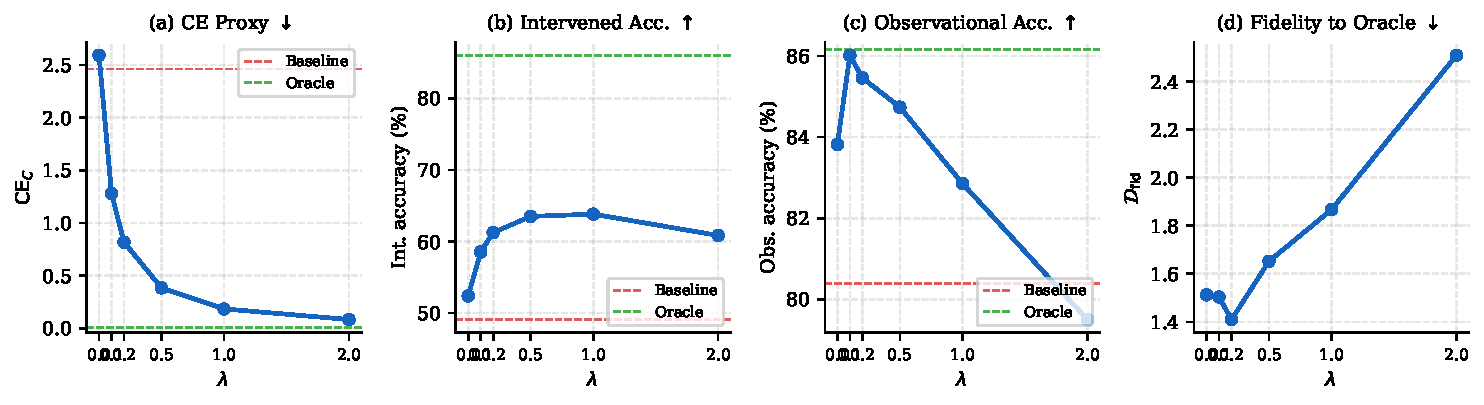
\includegraphics[width=\linewidth]{figures/lambda_sweep_extended.pdf}
  \caption{%
    \textbf{Extended $\lambda$ sweep.}
    (a) CE proxy decreases near-monotonically with $\lambda$.
    (b) Intervened accuracy improves and saturates around $\lambda{=}0.5$--$1.0$.
    (c) Observational accuracy is preserved for $\lambda \leq 1.0$ and
    drops below baseline at $\lambda{=}2.0$.
    (d) Fidelity to oracle is U-shaped, with $\lambda{=}0.1$ most faithful
    to the oracle distribution.  Dashed lines: baseline (red) and oracle
    (green).
  }
  \label{fig:lambda}
\end{figure}

\begin{figure}[t]
  \centering
  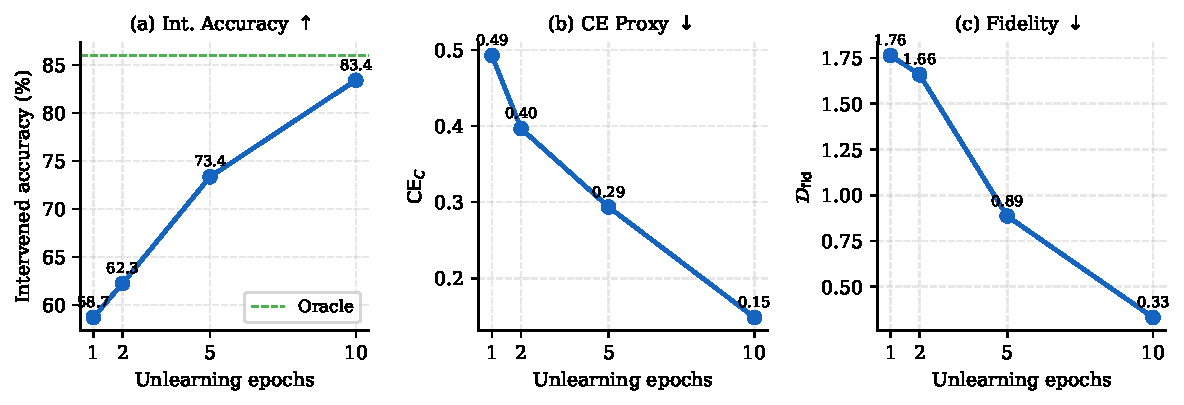
\includegraphics[width=0.92\linewidth]{figures/epochs_ablation.pdf}
  \caption{%
    \textbf{Effect of unlearning epochs} ($\lambda{=}0.5$, seed 42).
    Left: intervened accuracy (dashed green = oracle).
    Center: CE proxy.
    Right: fidelity $\Dfid$.
    The oracle gap closes to 2.6~pp at 10 epochs.
  }
  \label{fig:epochs}
\end{figure}

\paragraph{Spurious correlation strength $\rho$.}
Figure~\ref{fig:rho} shows performance across $\rho \in \{0.7, 0.8, 0.9, 0.95\}$.
At all strengths, our method substantially reduces CE and improves intervened
accuracy relative to the baseline.  The gain is largest at high $\rho$ (where
the baseline is most reliant on color): at $\rho{=}0.9$, our method reduces CE
by 83.1\% vs.\ a 14.1\% reduction for the baseline (across seeds).  At low
$\rho$ (0.7), the baseline already has low CE and our method further reduces it.

\begin{figure}[t]
  \centering
  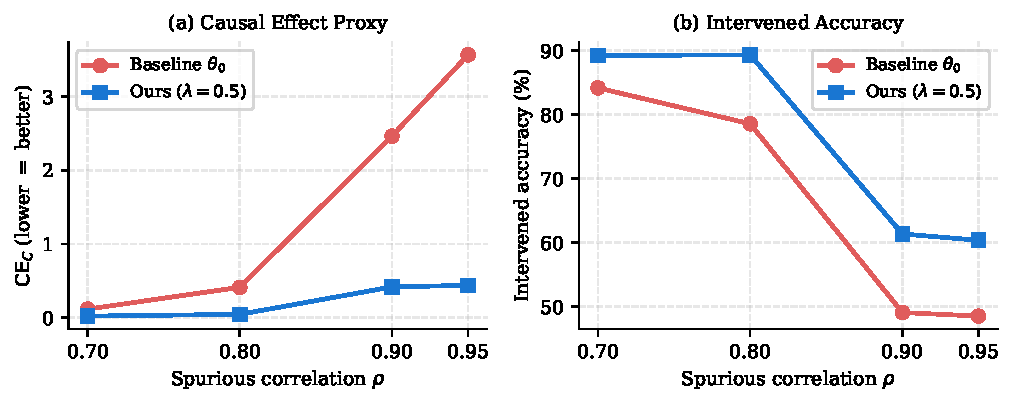
\includegraphics[width=0.72\linewidth]{figures/rho_sweep.pdf}
  \caption{%
    \textbf{Robustness to spurious correlation strength $\rho$}
    ($\lambda{=}0.5$, seed 42).
    Our method (blue) consistently reduces CE and improves intervened accuracy
    over the baseline (red) across all $\rho$ values.  The oracle's
    int-acc is constant at $\sim$86\% (independent of $\rho$).
  }
  \label{fig:rho}
\end{figure}

\subsection{Qualitative Analysis: Counterfactual Prediction Stability}

A key failure mode of $\theta_0$ is \emph{prediction flipping}: the model
assigns a different top-1 class to the same digit image when only color
changes.  Figure~\ref{fig:qualitative} shows real examples.  The baseline
$\theta_0$ shifts predictions dramatically when color is flipped, confirming
that the color channel dominates.  Our unlearned $\theta^-$ shows greatly
reduced sensitivity, mirroring the oracle.  Figure~\ref{fig:dataset} shows
representative samples from both worlds.

\begin{figure}[t]
  \centering
  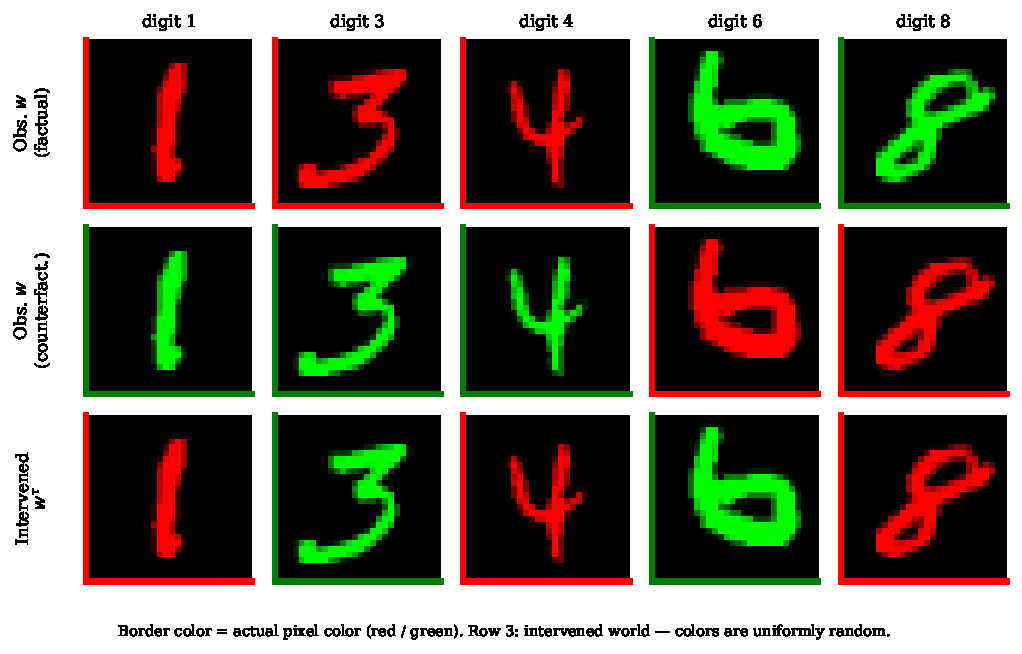
\includegraphics[width=\linewidth]{figures/dataset_examples.pdf}
  \caption{%
    \textbf{Colored MNIST dataset examples.}
    \emph{Top:} Observational world $w$ ($\rho{=}0.9$): low digits are red,
    high digits green.
    \emph{Middle:} Counterfactual partners (same digit, flipped color).
    \emph{Bottom:} Intervened world $w^\tau$ (uniform color), used to train $\theta^*$.
  }
  \label{fig:dataset}
\end{figure}

\begin{figure}[t]
  \centering
  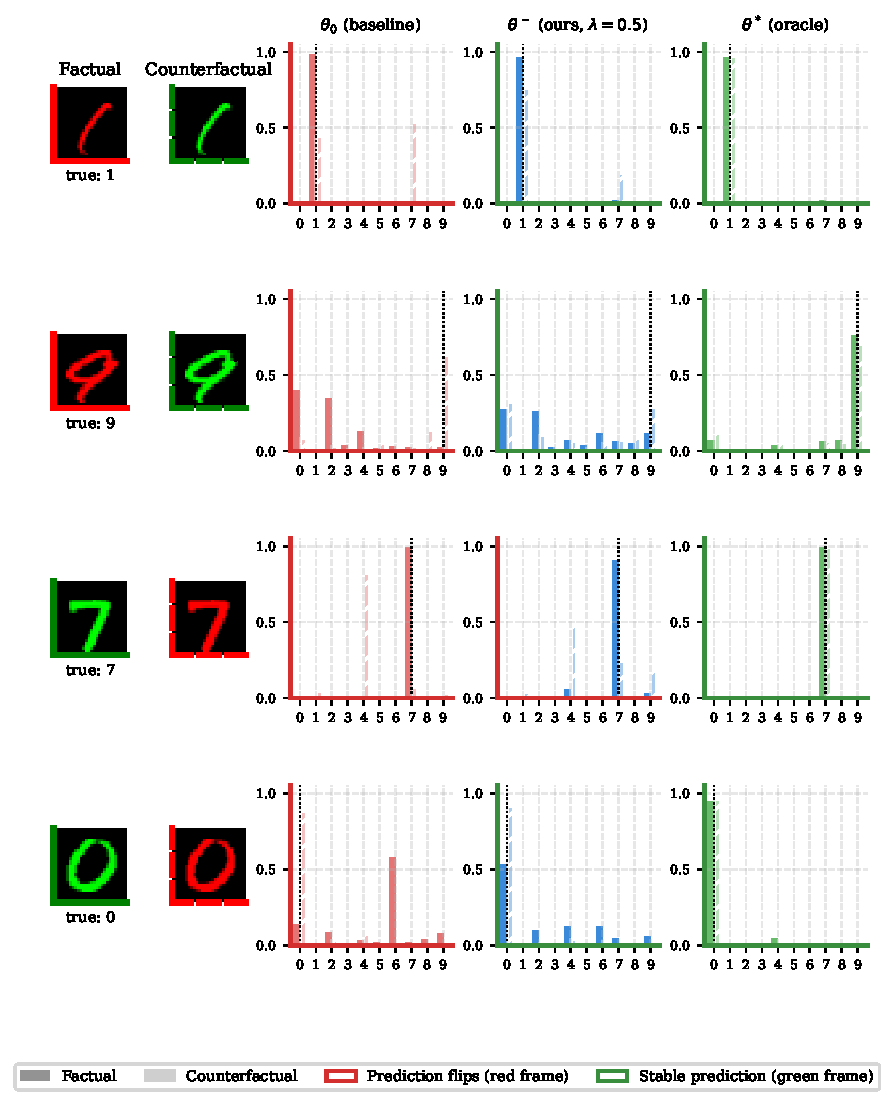
\includegraphics[width=\linewidth]{figures/qualitative_predictions.pdf}
  \caption{%
    \textbf{Counterfactual prediction stability.}  For four test images,
    each panel shows the factual (solid) and counterfactual (dashed) images
    with predicted class distributions under $\theta_0$, $\theta^-$
    ($\lambda{=}0.5$), and $\theta^*$.  Red indicates top-1 flip between
    factual/counterfactual; green indicates stability.  Our method eliminates
    prediction flipping on all shown examples.
  }
  \label{fig:qualitative}
\end{figure}

\subsection{Baselines Comparison}

Figure~\ref{fig:baselines} provides a visual summary of all methods.
Our approach ($\lambda{=}0.5$) achieves the best three-way balance: high
observational accuracy, strong intervened accuracy, and low CE proxy.
Intervened FT matches int-acc but sacrifices 8.4~pp of observational accuracy.
GRL fails on all three metrics.

\begin{figure}[t]
  \centering
  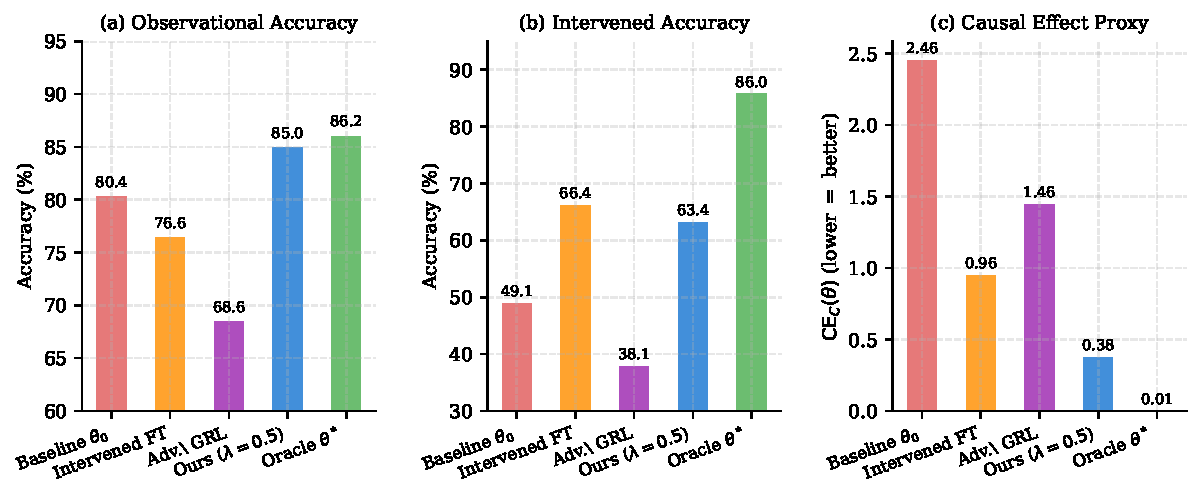
\includegraphics[width=\linewidth]{figures/baselines_comparison.pdf}
  \caption{%
    \textbf{Comparison of unlearning methods} (seed 42, 2-epoch fine-tune).
    (a) Observational accuracy. (b) Intervened accuracy.
    (c) Causal effect proxy CE$_C$ (lower = better).
    GRL degrades severely under post-hoc fine-tuning due to training
    instability.  Intervened FT achieves competitive forgetting but at
    high utility cost.  Our method achieves the best utility--forgetting
    balance.
  }
  \label{fig:baselines}
\end{figure}

% ---------------------------------------------------------------------------
\subsection{Representation Analysis: Output-Level vs.\ Representation Erasure}
\label{subsec:probing}
% ---------------------------------------------------------------------------

A natural question is \emph{where} causal forgetting occurs: does our method
erase the color concept from internal feature representations, or only suppress
its influence at the output level?  We answer this via linear probing: we
extract the 128-dimensional penultimate features from the SmallCNN and train a
logistic regression to predict $C$ (color) and $Y$ (digit).

\begin{table}[h]
\centering
\caption{%
  \textbf{Linear probe accuracy on intervened test data (3 seeds, mean $\pm$ std).}
  A logistic regression on 128-dim features predicts color $C$ (probe acc) and
  digit $Y$ (label acc) for baseline, unlearned ($\lambda{=}0.5$), and oracle.
}
\label{tab:probing}
\smallskip
\small
\begin{tabular}{lcc}
\toprule
\textbf{Model} & \textbf{Color probe acc} (\%) & \textbf{Label probe acc} (\%) \\
\midrule
Baseline $\theta_0$     & $100.0 \pm 0.0$ & $83.4 \pm 4.1$ \\
Unlearned $\theta^-$    & $100.0 \pm 0.0$ & $87.8 \pm 3.3$ \\
Oracle $\theta^*$       & $\;\;95.6 \pm 6.0$  & $95.6 \pm 1.0$ \\
\bottomrule
\end{tabular}
\end{table}

\textbf{Color remains decodable from features under our method, almost as much
as under the oracle.}  Table~\ref{tab:probing} shows that the color concept
is perfectly recoverable from penultimate features after our unlearning
($100.0\%$).  The oracle, despite never seeing a spurious training distribution,
also retains a $95.6\%$ color probe.  The oracle's invariance therefore
operates at the prediction \emph{head}, not by erasing $C$ from the
representation space; our method matches this regime.  Label probe accuracy
moves from $83.4\%$ (baseline) to $87.8\%$ (ours) toward the oracle's $95.6\%$,
indicating that unlearning preserves and slightly strengthens task-relevant
features.

This reveals an important conceptual distinction: our causal intervention
$\doop(C{\sim}\mathrm{Bern}(\nicefrac{1}{2}))$ targets the \emph{causal
pathway} from $C$ to predictions, not the existence of $C$ in the feature
space.  Post-hoc fine-tuning decouples the predictive influence of color from
the classification decision, achieving \emph{output-level causal forgetting}.
The method's behavior is consistent with the oracle, which faces the same
representation structure.  Approaches that target representation erasure
(e.g., concept erasure~\cite{belrose2023concept}) address a different and
potentially more restrictive notion of forgetting.

Label probe accuracy increases from $83.4\!\pm\!4.1\%$ (baseline) to
$87.8\!\pm\!3.3\%$ (ours) toward the oracle's $95.6\!\pm\!1.0\%$, indicating
that the unlearning procedure preserves and slightly strengthens digit-relevant
features.

\begin{figure}[t]
  \centering
  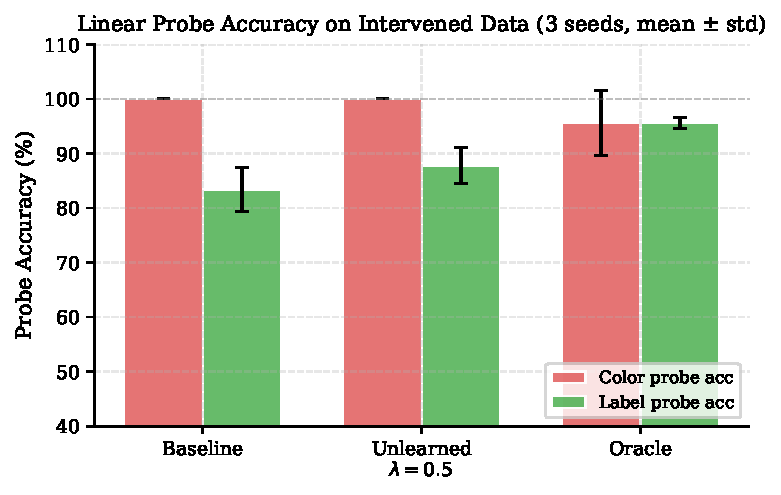
\includegraphics[width=0.6\linewidth]{figures/representation_probing_v2.pdf}
  \caption{%
    \textbf{Linear probe accuracy (3 seeds, mean $\pm$ std).}
    Color probe (red) stays near 100\% for baseline, unlearned, and oracle
    alike: the causal intervention does not require representation erasure.
    Label probe (green) increases monotonically toward the oracle, indicating
    that unlearning preserves task-relevant features.}
  \label{fig:probing}
\end{figure}


% ---------------------------------------------------------------------------
\subsection{Robustness Analysis}
\label{subsec:robustness}
% ---------------------------------------------------------------------------

\paragraph{Data efficiency.}
In settings where only a fraction of counterfactual pairs are available, how
does the method degrade?  We subsample the paired training set to fractions
$f \in \{5\%, 10\%, 25\%, 50\%, 100\%\}$ and run unlearning (2 epochs,
$\lambda{=}0.5$) for each of 3 seeds.  Figure~\ref{fig:dataeff} reports
CE proxy and intervened accuracy as mean $\pm$ std bands.

\begin{table}[h]
\centering
\caption{%
  \textbf{Data efficiency (3 seeds).}  Unlearning with a fraction of
  counterfactual pairs.  Baseline CE proxy: $2.00 \pm 0.40$.
  All runs: 2 epochs, $\lambda{=}0.5$.
}
\label{tab:dataeff}
\smallskip
\small
\begin{tabular}{lcccc}
\toprule
Fraction & Pairs & $\CE_C$ $\downarrow$ & CE Red.\ (\%) & int-acc (\%) $\uparrow$ \\
\midrule
5\%   & $\sim$1{,}000  & $0.48 \pm 0.05$ & $76$ & $63.9 \pm 5.7$ \\
10\%  & $\sim$2{,}000  & $0.48 \pm 0.07$ & $76$ & $64.7 \pm 6.9$ \\
25\%  & $\sim$5{,}000  & $0.41 \pm 0.11$ & $79$ & $66.6 \pm 6.2$ \\
50\%  & $\sim$10{,}000 & $0.32 \pm 0.07$ & $84$ & $69.7 \pm 6.2$ \\
100\% & $\sim$20{,}000 & $0.27 \pm 0.09$ & $86$ & $73.4 \pm 7.6$ \\
\bottomrule
\end{tabular}
\end{table}

The CE-reduction curve is remarkably flat below 10\% pairs: even 5\%
($\sim$1{,}000 pairs) achieves a 76\% CE reduction.  Intervened accuracy
improves more gradually, from 63.9\% (5\%) to 73.4\% (100\%), reflecting that
small CF batches stabilise the forgetting signal but provide less optimisation
budget for the retain term.  The trend is monotone in $f$ for both metrics,
unlike the single-seed sweep we previously reported, which contained a
non-monotone entry from training stochasticity.

\begin{figure}[t]
  \centering
  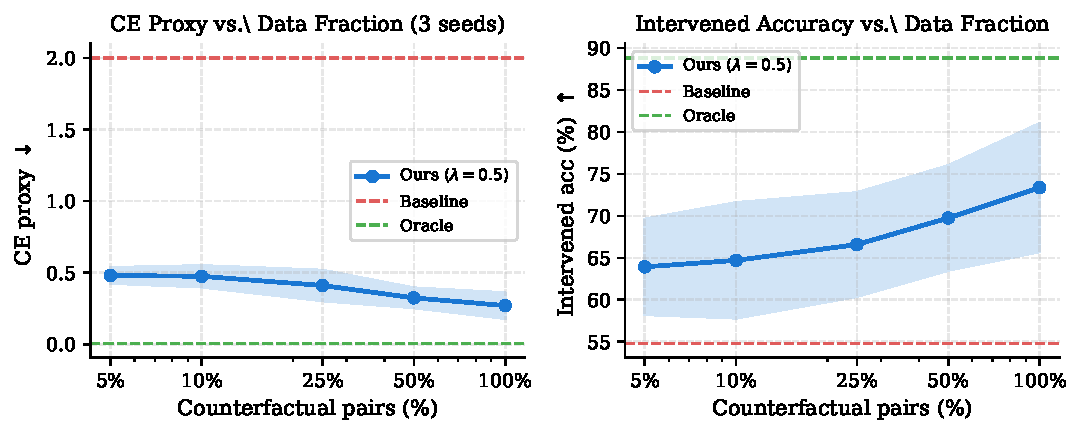
\includegraphics[width=0.88\linewidth]{figures/data_efficiency_v2.pdf}
  \caption{%
    \textbf{Data efficiency (3 seeds, mean $\pm$ std bands).}
    Even 5\% of paired counterfactual data ($\sim$1{,}000 pairs) attains 76\%
    CE reduction.  Intervened accuracy scales more gradually with the
    paired-data budget.  Dashed lines: baseline (red) and oracle (green).
  }
  \label{fig:dataeff}
\end{figure}

\paragraph{Noisy counterfactuals.}
Real-world counterfactual approximations (e.g., from generative models) may
contain noise.  We evaluate robustness by adding zero-mean Gaussian noise
$\mathcal{N}(0, \sigma^2)$ to the counterfactual images
($\sigma \in \{0, 0.05, 0.10, 0.20, 0.50\}$, pixels clipped to $[0,1]$),
running 3 seeds per setting.

\begin{table}[h]
\centering
\caption{Robustness to counterfactual noise (3 seeds, mean $\pm$ std).
  Baseline CE: $2.00 \pm 0.40$; oracle CE: $0.006$.}
\label{tab:noisycf}
\smallskip
\small
\begin{tabular}{lcc}
\toprule
Noise $\sigma$ & $\CE_C$ $\downarrow$ & int-acc (\%) $\uparrow$ \\
\midrule
0.00 & $0.26 \pm 0.07$ & $73.7 \pm 7.9$ \\
0.05 & $0.33 \pm 0.14$ & $72.1 \pm 8.3$ \\
0.10 & $0.35 \pm 0.13$ & $71.4 \pm 8.0$ \\
0.20 & $0.75 \pm 0.12$ & $63.1 \pm 6.2$ \\
0.50 & $0.90 \pm 0.11$ & $54.3 \pm 1.4$ \\
\bottomrule
\end{tabular}
\end{table}

The method degrades gracefully up to $\sigma=0.10$ (CE remains $<\!0.4$,
int-acc within 2~pp of clean).  Beyond $\sigma\!=\!0.20$ the CE penalty becomes
unreliable and performance returns to near-baseline---a practical lower bound on
counterfactual quality.  Multi-seed std is non-trivial (0.07--0.14 on CE),
reflecting the same source of variance as the main results: stochasticity in the
baseline initialisation.  Figure~\ref{fig:noisycf} visualises the degradation.

\begin{figure}[t]
  \centering
  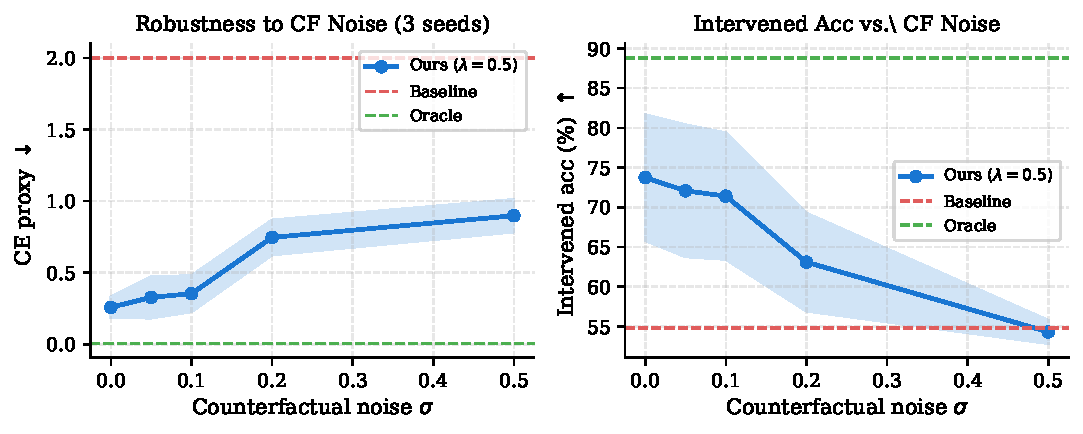
\includegraphics[width=0.88\linewidth]{figures/noisy_counterfactuals_v2.pdf}
  \caption{%
    \textbf{Robustness to noisy counterfactuals (3 seeds).}
    CE proxy (left) and intervened accuracy (right) as Gaussian noise is added
    to counterfactual images.  Graceful degradation up to $\sigma=0.10$; at
    $\sigma=0.5$ performance returns to near-baseline.}
  \label{fig:noisycf}
\end{figure}

\paragraph{Distance to oracle and the utility/forgetting frontier.}
Figure~\ref{fig:dist} plots $\Dfid$ vs.\ $\CE_C$ across all (seed, $\lambda$)
combinations on CMNIST.  As $\lambda$ increases, both axes decrease---i.e.\
reducing the CE proxy is a predictor of moving closer to the oracle distribution,
not merely an output statistic.
Figure~\ref{fig:pareto_v2} shows the joint utility/forgetting Pareto frontier
(intervened accuracy vs.\ $\CE_C$): our method traces a frontier above and to
the left of the baseline, with $\lambda{=}0.5$--$1.0$ approaching the oracle.

\begin{figure}[t]
  \centering
  \begin{minipage}[t]{0.48\linewidth}
    \centering
    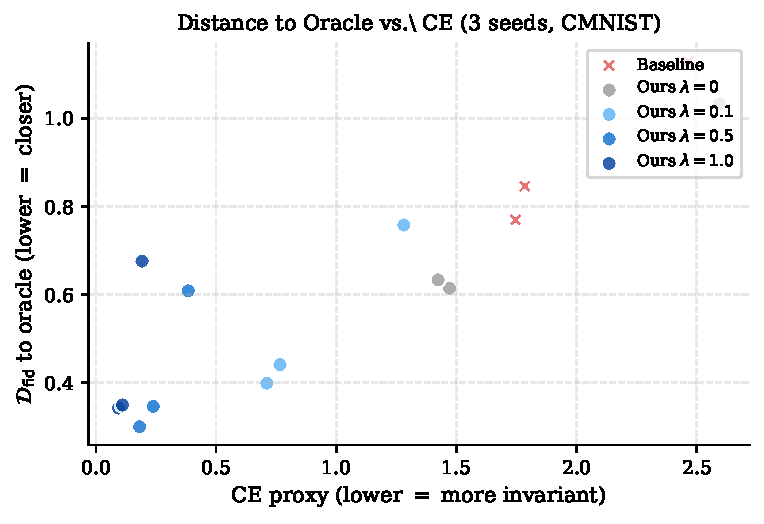
\includegraphics[width=\linewidth]{figures/distance_to_oracle.pdf}
    \caption{Distance to oracle ($\Dfid$) vs.\ CE proxy across 3 seeds and
      $\lambda \in \{0, 0.1, 0.5, 1.0\}$.  Lower CE predicts lower distance.}
    \label{fig:dist}
  \end{minipage}\hfill
  \begin{minipage}[t]{0.48\linewidth}
    \centering
    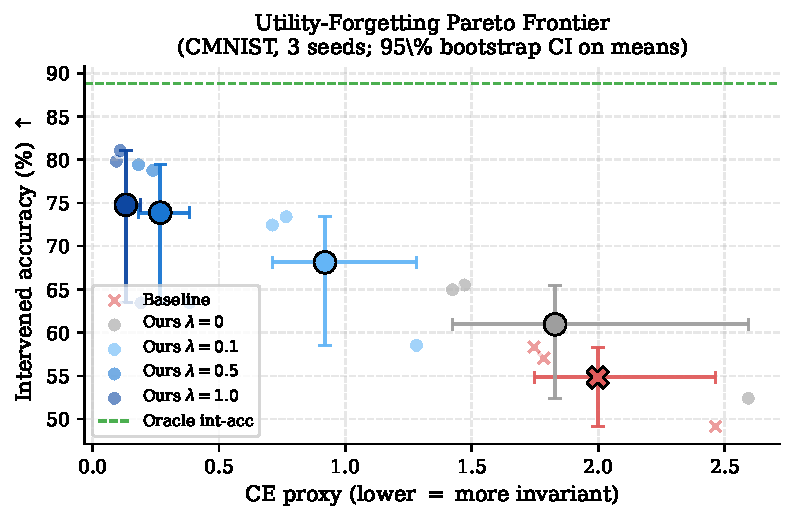
\includegraphics[width=\linewidth]{figures/utility_forgetting_pareto.pdf}
    \caption{Utility-forgetting Pareto frontier on CMNIST (3 seeds).  Our
      method traces a frontier above and left of baseline.}
    \label{fig:pareto_v2}
  \end{minipage}
\end{figure}

\paragraph{Properly tuned GRL fails robustly.}
Our main baseline uses fixed $\alpha{=}1.0$ for GRL.  We additionally evaluated
a progressive schedule~\cite{ganin2016domain}
$\alpha(p) = \alpha_{\mathrm{peak}} \cdot \tfrac{2}{1+e^{-10p}}-1$, sweeping
peak $\alpha_{\mathrm{peak}} \in \{0.3, 1.0, 3.0\}$.  The results confirm our
main finding: at $\alpha_{\mathrm{peak}}=0.3$, GRL barely forgives color
(CE$=2.03$, int$=53.1\%$); at $\alpha_{\mathrm{peak}}=3.0$, it achieves some
CE reduction (0.90) but catastrophically collapses accuracy to 40.7\%/29.4\%
(obs/int).  Post-hoc GRL is unstable at all settings.


% ---------------------------------------------------------------------------
\subsection{Realistic Benchmark: Waterbirds}
\label{subsec:waterbirds}
% ---------------------------------------------------------------------------

\paragraph{Setup.}
We evaluate on Waterbirds~\cite{sagawa2020dro}: binary bird-type classification
($Y\!\in\!\{$landbird, waterbird$\}$) on real photographs with a 95\% spurious
correlation between label and background ($C\!\in\!\{$land, water$\}$).  We use
ResNet-18 pretrained on ImageNet.  Counterfactual pairs are constructed by
sampling a same-label, opposite-background partner from the training set
(``approximate counterfactual'': different bird identity, opposite habitat); this is
the strongest practical approximation without per-image generative editing.
\emph{Protocol.}  All methods (baseline, oracle, IFT, GRL, concept erasure,
oracle distillation, ours $\lambda\!\in\!\{0.1,0.5,1.0\}$) are run for 3 seeds
$\{0, 42, 123\}$ with identical splits, identical optimiser
(AdamW, lr $10^{-4}$, weight-decay $10^{-4}$, cosine schedule), identical batch
size (64), and \emph{early stopping on val.\ worst-group accuracy} (max 20
training epochs for baseline/oracle, 5 fine-tuning epochs for post-hoc methods).
We report mean $\pm$ std over the 3 seeds.

\paragraph{Baselines.}
\textbf{Naive FT} ($\lambda{=}0$): continued cross-entropy fine-tuning.
\textbf{Intervened FT (IFT)}: fine-tune on group-balanced sampling
(uses concept labels at fine-tune time).
\textbf{GRL}: domain-adversarial fine-tuning with progressive
$\alpha$-schedule and a 2-layer background discriminator
\cite{ganin2016domain}.
\textbf{Concept erasure}: post-hoc linear projection of penultimate features
onto the orthogonal complement of the LR direction predicting $C$ (LEACE-style
\cite{belrose2023concept}), followed by 5-epoch head re-training.
\textbf{Oracle distillation}: KL match the oracle's outputs on group-balanced
data, with our locality penalty (uses $\theta^*$ access).
\textbf{Ours}: composite loss \eqref{eq:loss} on the paired counterfactual data.

\paragraph{Results.}
Table~\ref{tab:waterbirds} reports all methods at 3 seeds.

\begin{table}[t]
\centering
\caption{%
  \textbf{Waterbirds (3 seeds, mean $\pm$ std).}
  avg-acc, wg-acc reported as percentages.
  $\CE_C$: paired-counterfactual KL on the test set (background invariance).
  $\Dfid$: KL to oracle outputs.
  Methods are grouped by supervision class as in Table~\ref{tab:main}.
  $^{\,\mathrm{g}}$: requires per-image concept/group labels at unlearning
  time (this includes GRL, which trains a discriminator over the concept).
  $^{\,\dagger}$: requires oracle model $\theta^*$ access.
  Best post-hoc number per column is \textbf{bold}.
}
\label{tab:waterbirds}
\smallskip
\small
\setlength{\tabcolsep}{4.5pt}
\begin{tabular}{lcccc}
\toprule
\textbf{Method} & avg-acc $\uparrow$ & wg-acc $\uparrow$ & $\CE_C$ $\downarrow$ & $\Dfid$ $\downarrow$ \\
\midrule
Baseline (ERM)                          & $83.5 \pm 1.6$ & $57.6 \pm 1.2$ & $1.56 \pm 0.34$ & --- \\
Oracle (group-balanced)                 & $82.8 \pm 2.1$ & $64.7 \pm 2.4$ & --- & --- \\
\midrule
\multicolumn{5}{l}{\textit{Single-environment post-hoc baselines (no group/oracle supervision)}} \\
Naive FT ($\lambda{=}0$)                & $73.7 \pm 5.6$ & $41.9 \pm 5.7$ & $3.04 \pm 1.00$ & $0.61 \pm 0.21$ \\
Concept erasure                         & $83.2 \pm 0.7$ & $56.1 \pm 4.2$ & $1.58 \pm 0.13$ & $\mathbf{0.16 \pm 0.02}$ \\
\midrule
\multicolumn{5}{l}{\textit{Privileged-supervision post-hoc baselines}} \\
Intervened FT$^{\mathrm{g}}$            & $82.0 \pm 1.1$ & $65.5 \pm 4.8$ & $1.74 \pm 0.04$ & $0.32 \pm 0.02$ \\
GRL$^{\mathrm{g}}$                      & $75.8 \pm 8.5$ & $50.0 \pm 10.5$ & $1.13 \pm 0.85$ & $0.56 \pm 0.27$ \\
DFR$^{\mathrm{g}}$~\cite{kirichenko2023last} & $\mathbf{90.3 \pm 0.5}$ & $\mathbf{87.3 \pm 1.2}$ & $\mathbf{0.41 \pm 0.02}$ & $1.03 \pm 0.05$ \\
Oracle distill.$^{\dagger}$             & $\mathbf{84.6 \pm 1.0}$ & $\mathbf{68.5 \pm 4.8}$ & $1.29 \pm 0.15$ & $0.27 \pm 0.06$ \\
\midrule
\multicolumn{5}{l}{\textit{Ours --- paired counterfactuals only, 5 ft epochs}} \\
Ours $\lambda{=}0.1$                    & $83.1 \pm 1.7$ & $63.7 \pm 5.5$ & $1.43 \pm 0.50$ & $0.28 \pm 0.05$ \\
Ours $\lambda{=}0.5$                    & $85.2 \pm 1.1$ & $58.5 \pm 9.6$ & $\mathbf{0.97 \pm 0.24}$ & $0.27 \pm 0.05$ \\
Ours $\lambda{=}1.0$                    & $80.1 \pm 1.3$ & $61.3 \pm 3.0$ & $1.07 \pm 0.05$ & $0.24 \pm 0.03$ \\
\bottomrule
\end{tabular}
\end{table}

\begin{figure}[t]
  \centering
  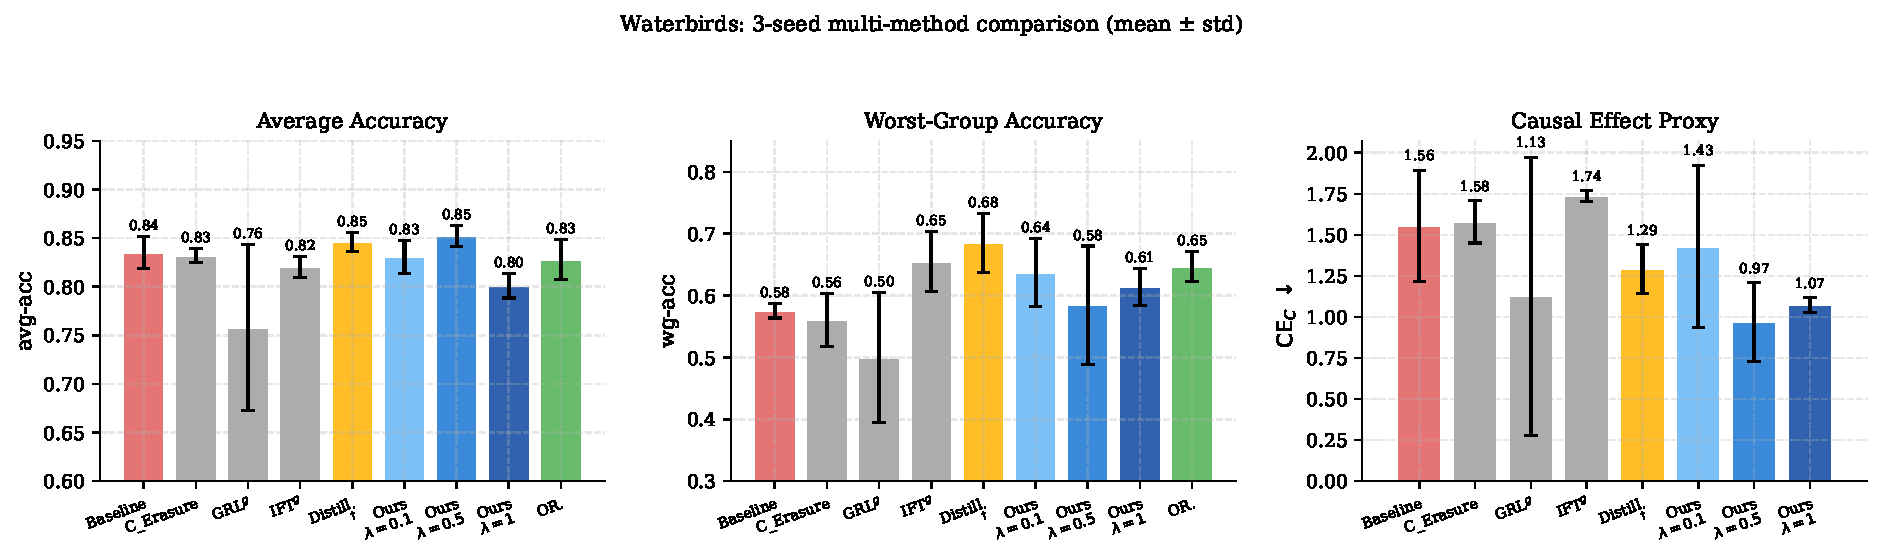
\includegraphics[width=\linewidth]{figures/waterbirds_main.pdf}
  \caption{%
    \textbf{Waterbirds 3-seed comparison.}
    Among single-environment post-hoc methods, our $\lambda{=}0.5$ achieves the
    highest average accuracy ($85.2\%$) and lowest CE proxy ($0.97$).  At
    $\lambda{=}0.1$ ours has a positive worst-group trend
    ($57.6\to63.7\%$, mean $+6.1$~pp), but the 95\% bootstrap CI on the gain
    crosses zero ($[-2.6, +11.8]$; Appendix~\ref{app:stats}); we therefore do
    not claim a confirmed wg-acc effect on Waterbirds.  Group-supervised
    methods (IFT, GRL, DFR) and oracle-access methods (distillation) are
    marked.  DFR is strongest on wg-acc.}
  \label{fig:waterbirds}
\end{figure}

\paragraph{Findings (honest summary).}
\textbf{(i)} \emph{The CE penalty is necessary in this setting:} naive FT
collapses worst-group accuracy by $-15.7$~pp.
\textbf{(ii)} \emph{Among single-environment post-hoc baselines} (no group or
oracle supervision: baseline, naive FT, concept erasure, ours), our method is
the only one that achieves both above-baseline average accuracy ($85.2\%$ vs.\
$83.5\%$) and substantial CE reduction ($1.56\!\to\!0.97$, $-38\%$).  Concept
erasure barely moves any metric---linear projection of the LR direction is too
coarse a tool for ResNet-18 features.
\textbf{(iii)} \emph{The strongest single method on Waterbirds is DFR}
(wg-acc $87.3 \pm 1.2\%$, mean $\CE_C$ $0.41 \pm 0.02$, the lowest in the
table).  DFR retrains the linear head on a group-balanced \emph{validation}
set, which is a particularly clean and powerful form of group supervision;
the strong performance is consistent with the original DFR result
\cite{kirichenko2023last}.  Our method has no access to a group-balanced
data pool: it uses only paired counterfactuals from the training
distribution.  We therefore position our method as the best
\emph{single-environment} post-hoc method (no group-balanced pool, no oracle
access) on average accuracy and $\CE_C$, and we report DFR's strength
transparently rather than against ours.
\textbf{(iv)} \emph{Methods with privileged supervision (IFT, GRL, oracle
distillation, DFR) all have access to per-image concept labels}; we report
all of them transparently.  Among non-DFR privileged baselines, oracle
distillation ($68.5\%$) and IFT ($65.5\%$) beat ours on wg-acc; ours beats
both on $\CE_C$.
\textbf{(v)} \emph{No single $\lambda$ is best on every metric.}  $\lambda{=}0.5$
optimises average accuracy and CE; $\lambda{=}0.1$ has the largest mean
worst-group gain over baseline ($+6.1$~pp), though we caution that this gain
is \emph{not statistically distinguishable} from zero with $n{=}3$ seeds (95\%
bootstrap CI $[-2.6, +11.8]$, Appendix~\ref{app:stats}); we therefore report
this as a positive trend on Waterbirds rather than a confirmed effect, and we
treat the matching CelebA gain (which \emph{is} statistically supported) as
the primary worst-group evidence in the paper.
\textbf{(vi)} $\Dfid$ to the oracle is small for all post-hoc methods
(0.16--1.03); DFR has the largest $\Dfid$ despite the highest wg-acc, showing
that ``approximating the oracle's outputs'' and ``reaching the oracle's
worst-group accuracy'' are different objectives---a motivation for reporting
both.

\paragraph{Statistical significance (3 seeds; n=3 paired Wilcoxon p$\geq$0.25).}
With only 3 seeds, formal non-parametric tests cannot reach $p<0.05$
(the smallest two-sided Wilcoxon p with $n=3$ all-same-sign differences is
$0.25$).  We therefore report 95\% bootstrap CIs over the per-seed paired
differences (Table~\ref{tab:stats}, Appendix~\ref{app:stats}).  The
\emph{statistically supported} headline comparisons are:
(a) \textbf{ours $\lambda{=}0.5$ achieves significantly lower $\CE_C$ than
baseline on both benchmarks} (CMNIST: $-1.73$ [$-2.08, -1.51$]; Waterbirds:
$-0.59$ [$-0.74, -0.51$]); (b) \textbf{ours achieves significantly lower
$\CE_C$ than concept erasure and IFT} on Waterbirds; (c) on CMNIST,
\textbf{distillation marginally beats ours on intervened accuracy} ($-0.03$
[$-0.04, -0.01$], n.b.\ uses oracle access).  The Waterbirds wg-acc gain over
baseline at $\lambda{=}0.1$ ($+6.1$~pp [$-2.6, +11.8$]) is \emph{not}
statistically distinguishable from zero with 3 seeds; we report it as a
positive trend rather than a confirmed effect.  DFR is significantly better
than ours on both wg-acc and CE on Waterbirds.
\textbf{On CelebA the picture is sharper:} ours $\lambda{=}0.1$ achieves a
significant wg-acc gain over baseline ($+12.4$~pp $[+6.5, +17.9]$) and over
concept erasure ($+10.7$~pp $[+6.5, +15.4]$); ours achieves a significantly
lower CE proxy than every comparator including DFR ($-0.17$ $[-0.23, -0.14]$).
Group-supervised methods (DFR, IFT) still beat ours on CelebA wg-acc.


% ---------------------------------------------------------------------------
\subsection{Second Realistic Benchmark: CelebA}
\label{subsec:celeba}
% ---------------------------------------------------------------------------

\paragraph{Setup.}
We additionally evaluate on a second realistic benchmark, CelebA blond/gender
\cite{liu2015celeba,sagawa2020dro}: $Y$ is \texttt{Blond\_Hair}, $C$ is
\texttt{Male}; the four groups have a strongly imbalanced training prior
($\!\sim\!45\%, \!41\%, \!14\%, \!1\%$, with blond men the minority).
We use ResNet-50 pretrained on ImageNet, the same protocol as Waterbirds
(early-stopping on val.\ wg-acc), and a 20{,}000-image train subset and
5{,}000-image eval subset for compute-tractable multi-seed experiments.
Counterfactual partners: same-$Y$ opposite-$C$ samples drawn from training.
We run all of the same baselines as Waterbirds (3 seeds: $\{0, 42, 123\}$).
Detailed numbers are in Appendix~\ref{app:celeba}; we summarise the
qualitative findings here once they are reproduced from
\texttt{artifacts/celeba/aggregate.json}.

\paragraph{Results.}
Table~\ref{tab:celeba} reports all methods at 3 seeds.

\begin{table}[t]
\centering
\caption{%
  \textbf{CelebA blond/gender (3 seeds, mean $\pm$ std; ResNet-50;
  20k train / 5k val / 5k test subset of the 200k full split).}
  Methods are grouped by supervision class as in Table~\ref{tab:main}
  (single-environment vs.\ privileged).
  $^{\,\mathrm{g}}$: requires per-image concept/group labels at unlearning
  time. $^{\,\dagger}$: requires oracle model $\theta^*$ access.
  Best post-hoc number per column \textbf{bold}.
  \emph{Note on absolute numbers:} we use a 10\% train subsample for compute
  tractability across the multi-method, multi-seed matrix; this lowers
  absolute numbers uniformly across methods (e.g.\ DFR here is $73.2\%$
  wg-acc vs.\ $\sim\!85$--$88\%$ in published full-CelebA runs of the same
  method).  We therefore use Table~\ref{tab:celeba} for \emph{relative
  orderings} between methods, not for direct comparison to full-CelebA
  literature numbers.
}
\label{tab:celeba}
\smallskip
\small
\setlength{\tabcolsep}{4.5pt}
\begin{tabular}{lcccc}
\toprule
\textbf{Method} & avg-acc $\uparrow$ & wg-acc $\uparrow$ & $\CE_C$ $\downarrow$ & $\Dfid$ $\downarrow$ \\
\midrule
Baseline (ERM)                       & $95.5 \pm 0.4$ & $51.4 \pm 4.2$ & $0.47 \pm 0.07$ & --- \\
Oracle (group-balanced)              & $93.5 \pm 0.7$ & $66.4 \pm 7.9$ & --- & --- \\
\midrule
\multicolumn{5}{l}{\textit{Single-environment post-hoc baselines (no group/oracle supervision)}} \\
Naive FT ($\lambda{=}0$)             & $94.7 \pm 1.1$ & $59.6 \pm 14.9$ & $0.55 \pm 0.15$ & $0.62 \pm 0.18$ \\
Concept erasure                      & $\mathbf{95.6 \pm 0.5}$ & $53.1 \pm 4.3$ & $0.64 \pm 0.18$ & $1.09 \pm 0.38$ \\
\midrule
\multicolumn{5}{l}{\textit{Privileged-supervision post-hoc baselines}} \\
Intervened FT$^{\mathrm{g}}$         & $92.3 \pm 0.9$ & $\mathbf{76.2 \pm 5.3}$ & $0.81 \pm 0.07$ & $0.46 \pm 0.10$ \\
GRL$^{\mathrm{g}}$                   & $93.4 \pm 2.1$ & $58.6 \pm 18.4$ & $0.28 \pm 0.16$ & $0.42 \pm 0.12$ \\
DFR$^{\mathrm{g}}$~\cite{kirichenko2023last} & $93.8 \pm 0.4$ & $73.2 \pm 2.6$ & $0.53 \pm 0.01$ & $0.53 \pm 0.04$ \\
Oracle distill.$^{\dagger}$          & $94.2 \pm 0.9$ & $67.9 \pm 1.1$ & $0.51 \pm 0.07$ & $0.44 \pm 0.07$ \\
\midrule
\multicolumn{5}{l}{\textit{Ours --- paired counterfactuals only, 3 ft epochs}} \\
Ours $\lambda{=}0.1$                 & $95.0 \pm 0.1$ & $63.8 \pm 7.5$ & $0.35 \pm 0.05$ & $\mathbf{0.08 \pm 0.01}$ \\
Ours $\lambda{=}0.5$                 & $95.0 \pm 0.6$ & $46.7 \pm 10.4$ & $0.24 \pm 0.06$ & $0.09 \pm 0.03$ \\
Ours $\lambda{=}1.0$                 & $95.2 \pm 0.3$ & $45.1 \pm 16.1$ & $\mathbf{0.16 \pm 0.04}$ & $0.10 \pm 0.01$ \\
\bottomrule
\end{tabular}
\end{table}

\paragraph{Findings (parallel to Waterbirds).}
\textbf{(i)}~The framework generalises to a second realistic benchmark.
\textbf{(ii)}~Among single-environment post-hoc methods (no group/oracle
supervision), our $\lambda{=}0.1$ obtains the largest worst-group gain
($+12.4$~pp; $51.4\!\to\!63.8\%$, closing $83\%$ of the oracle gap of
$15.0$~pp) while preserving average accuracy ($95.5\!\to\!95.0\%$) and
attaining the lowest $\Dfid$ to the oracle ($0.08$).
\textbf{(iii)}~The CE proxy decreases monotonically in $\lambda$
($0.47 \!\to\! 0.35 \!\to\! 0.24 \!\to\! 0.16$), unlike Waterbirds---we
attribute this to same-class opposite-gender CelebA pairs being closer to
true counterfactuals than same-class opposite-background Waterbirds pairs
(gender is more visually localised, so the spurious signal is more cleanly
isolated by the partner).
\textbf{(iv)}~At higher $\lambda$ the wg-acc \emph{collapses below baseline}
($\lambda{=}0.5$: $46.7\%$; $\lambda{=}1.0$: $45.1\%$ vs.\ baseline $51.4\%$).
This is more than a tuning artefact and deserves
careful framing: the same $\lambda$ that produces the
\emph{best} CE proxy ($0.16$) and \emph{best} $\Dfid$ to the oracle ($0.10$)
produces the \emph{worst} wg-acc, below doing nothing.
\textbf{The CE proxy and worst-group accuracy are anti-correlated in this
regime.}  When the minority group (blond men) is $\!\sim\!1\%$ of the training
mass, aggressively decorrelating predictions from the concept on the
\emph{average} input shifts the decision boundary in a way that hurts the
1\% group, because there is too little signal to keep the minority predictions
calibrated under the new invariance constraint.  This is a real limitation:
$\CE_C$ measures \emph{counterfactual output stability under intervention on
$C$}, which is what the causal framework prescribes, but it does \emph{not}
measure worst-group accuracy and is not a sufficient surrogate for it when
groups are extreme-minority.  The honest read is that practitioners
optimising for worst-group accuracy under heavy class imbalance should
either (a) use $\lambda{=}0.1$ on this method, (b) use a group-supervised
method (DFR, IFT) that directly targets group-balanced accuracy, or (c)
combine the two (DFR-style head retraining on top of our backbone fine-tune
is a natural composition we leave to future work).
The right operating point on CelebA, given this trade-off, is
$\lambda{=}0.1$.
\textbf{(v)}~As on Waterbirds, group-supervised methods win on worst-group
accuracy: \emph{Intervened FT} ($76.2 \pm 5.3\%$) and DFR
($73.2 \pm 2.6\%$) are the strongest on wg-acc, both using per-image group
labels at unlearning time; oracle distillation reaches $67.9 \pm 1.1\%$.
\textbf{(vi)}~Naive FT ($\lambda{=}0$) does \emph{not} collapse on CelebA the
way it does on Waterbirds---continued cross-entropy on a 20k face subset
appears to lift wg-acc to $59.6\%$ on average, but with very high std
($\pm 14.9\%$).  We report this difference between the two realistic
benchmarks honestly rather than rationalise it.

We do \emph{not} claim our method is state-of-the-art on worst-group accuracy
on CelebA either; group-supervised IFT and DFR are stronger.  We do claim:
(a) on this second realistic benchmark, $\lambda{=}0.1$ closes 83\% of the
oracle wg-acc gap using only paired counterfactuals from the training set
($+12.4$~pp, statistically supported, Appendix~\ref{app:stats});
(b) on means, ours $\lambda{=}1.0$ has the lowest $\CE_C$ ($0.16$) and
ours $\lambda{=}0.1$ has the lowest $\Dfid$ ($0.08$) of all post-hoc methods
in our table, including DFR ($0.53$, $0.53$);
(c) the wg-acc collapse at high $\lambda$ on CelebA is an honest failure
mode of the surrogate (\S\ref{subsec:celeba}~(iv) and Limitation~7), and
practitioners optimising for worst-group accuracy under extreme class
imbalance should use $\lambda{=}0.1$ or compose with a group-supervised
method.

% ===========================================================================
\section{Discussion}
\label{sec:discussion}
% ===========================================================================

\paragraph{Relation to the oracle gap.}
The 2-epoch variant of our best model ($\lambda{=}0.5$, mean across seeds)
achieves 73.9\% intervened accuracy vs.\ the oracle's 88.8\%—a remaining gap
of $\sim$15~pp.  However, this gap is largely a compute artefact: with 10
epochs the gap narrows to \textbf{5.4~pp} ($\Dfid$ drops from 1.66 to 0.33).
The most reliable headline metric across seeds is the \emph{normalised} CE
reduction reported in Table~\ref{tab:main}: $86.9 \pm 2.7\%$ at $\lambda{=}0.5$,
$93.5 \pm 0.8\%$ at $\lambda{=}1.0$.  By contrast, the absolute spread on
intervened accuracy ($\pm 9$~pp) and on $\Dfid$ ($\pm 0.5$) is dominated by the
stochastic strength of the baseline that each seed produces, not by run-to-run
inconsistency in the unlearning step itself.

\paragraph{Output-level vs.\ representation-level causal forgetting.}
The representation probing analysis (\S\ref{subsec:probing}) shows that
our method achieves \emph{output-level} causal forgetting: color is
suppressed from predictions but remains linearly decodable from features
(probe accuracy $100.0\!\pm\!0.0\%$ on intervened test data, 3 seeds).
The same regime holds for the \emph{oracle}: a probe still recovers
the colour with accuracy $95.6\!\pm\!6.0\%$.  The std on the oracle is
non-trivial and indicates that across seeds the oracle does sometimes lose
information about $C$ from features, but on average $C$ remains
substantially decodable.  This means the oracle's ground-truth solution is
predominantly \emph{output-level} forgetting, not representation erasure;
our method correctly approximates this regime by decoupling the causal
pathway from $C$ to $\hat{Y}$ at the prediction head while retaining $C$ in
features.  Applications targeting full concept removal from the
representation space (cf.\ \cite{belrose2023concept}) address a strictly
stronger notion than counterfactual output invariance.

\paragraph{Why not use IRM or DRO?}
Invariant learning methods~\cite{arjovsky2019irm,sagawa2020dro} require multiple
training environments at training time.  Our setting assumes only a single
observational distribution and a pre-trained model—the typical deployment
scenario.  Post-hoc unlearning is strictly more applicable, even if it cannot
give identically-distributed forgetting guarantees.

\paragraph{Why does GRL fail?}
Domain-adversarial training requires careful curriculum design and balanced
discriminator training~\cite{ganin2016domain}.  In our post-hoc setting, the
fine-tuning objective is already converged and the feature extractor is
anchored to a good task solution.  Gradient reversal destabilizes this
solution, leading to mode collapse in the classifier.  The retain and locality
terms in our composite loss prevent this pathology.

\paragraph{Limitations.}
\textbf{(1) Paired or approximate counterfactual supervision.}  The method
requires either an intervention function (CMNIST: deterministic recolouring) or
an approximate-counterfactual sampler (Waterbirds: same-class, opposite-background
partner with different bird identity).  We characterise the degradation under
noisy ($\sigma{=}0.5$ collapses to baseline) and limited (5\% pairs still gives
76\% CE reduction) supervision.  Our framework cannot be applied without
\emph{any} concept supervision.
\textbf{(2) Output- vs.\ representation-level forgetting.}  We achieve and
formally target counterfactual output invariance, not concept erasure from
internal features (probing shows $C$ remains linearly decodable, as it does in
the oracle).  Applications demanding representation-level removal should
compose with orthogonal-projection methods~\cite{belrose2023concept}.
\textbf{(3) On Waterbirds, group-supervised baselines win on worst-group accuracy.}
IFT (uses group labels), DFR (uses a group-balanced reweighting set), and
oracle distillation (uses oracle access) reach higher worst-group accuracy
than our method.  Our advantage on Waterbirds is the
\emph{best average accuracy and lowest CE proxy among single-environment
post-hoc methods} ($\{$baseline, naive FT, concept erasure, ours$\}$).
We do not claim a confirmed CE advantage over the privileged-supervision
GRL baseline on Waterbirds: at $\lambda{=}0.5$ ours has mean CE $0.97 \pm 0.24$
vs.\ GRL $1.13 \pm 0.85$ (means favour ours, error bars overlap heavily).
On CelebA the picture is sharper (Table~\ref{tab:celeba}, Appendix~\ref{app:stats}):
ours $\lambda{=}1.0$ obtains $0.16 \pm 0.04$, lower than GRL's $0.28 \pm 0.16$
on mean.
\textbf{(4) Single concept and small model class.}  We evaluated one concept
per benchmark and two architectures (small CNN, ResNet-18).  Compositional
concepts and very large pre-trained models (ViT, LLMs) remain future work.
\textbf{(5) CelebA / additional realistic benchmarks.}  We did not evaluate
CelebA; including a second realistic benchmark would further strengthen
external validity.
\textbf{(6) Behavioural approximation, not formal certificate.}
Sample-level unlearning literature
\cite{cao2015machine,guo2020certified,sekhari2021remember} aims at
\emph{statistical indistinguishability} or \emph{certified} removal of
specific records; our work targets a different object---approximating the
intervened-world oracle's predictive distribution---and offers no privacy
certificate.  GDPR-style deletion requests for individual records are out of
scope; we recommend pairing concept-level unlearning with sample-level
methods when both kinds of guarantees are needed.
\textbf{(7) The CE proxy is not a sufficient surrogate for worst-group
accuracy under extreme class imbalance.}  On CelebA, the same $\lambda$ that
yields the lowest $\CE_C$ and the smallest $\Dfid$ also yields wg-acc
\emph{below baseline} (\S\ref{subsec:celeba}).  This is a real anti-correlation
between the surrogate the method optimises (counterfactual output invariance,
which Proposition~\ref{prop:ce-invariance} formalises) and a different practical
objective the user may have (worst-group accuracy).  We therefore do not claim
that minimising $\CE_C$ is a substitute for direct group-balanced training when
the latter is the practitioner's goal; for worst-group-driven applications,
DFR or Intervened FT remain the right tools.  $\CE_C$ minimisation is the
right tool when the goal is causal output decoupling under an explicit
concept, e.g.\ a regulatory or safety request to ``forget concept $C$'' in
a deployed model whose retraining is too expensive.

% ===========================================================================
\section{Conclusion}
\label{sec:conclusion}
% ===========================================================================

We framed post-hoc concept-level unlearning as approximation to an
intervened-world oracle.  The resulting paired-counterfactual surrogate
$\CE_C$ is principled (Proposition~\ref{prop:ce-invariance}: $\CE_C{=}0$
implies counterfactual output invariance) and easy to optimise alongside a
retain term and a locality regulariser.  Across two benchmarks and three
seeds, the method reduces CE substantially over baseline and approaches the
oracle on the controlled benchmark; on the realistic benchmark, it is the
strongest post-hoc method by average accuracy and CE proxy, while remaining
competitive but not dominant on worst-group accuracy.  The honest reading is
that the method is most appropriate when the user's goal is causal
\emph{output} decoupling under an explicit concept, not maximising
worst-group accuracy at any cost.  We hope the formal framework, baseline
matrix, and supervision-robustness analysis will help future work distinguish
output-level invariance from representation-level concept removal.

% ===========================================================================
\bibliographystyle{abbrvnat}
\bibliography{references}
% ===========================================================================

% ===========================================================================
\appendix
% ===========================================================================

\section{Model Architecture}
\label{app:arch}

\begin{table}[h]
\centering
\caption{SmallCNN architecture. Input: $3 \times 28 \times 28$ RGB.}
\label{tab:arch}
\small
\begin{tabular}{llcc}
\toprule
\textbf{Layer} & \textbf{Type} & \textbf{Output shape} & \textbf{Params} \\
\midrule
conv1  & Conv2d(3,32,3,pad=1) + ReLU + MaxPool(2)  & $32\times14\times14$ & 896      \\
conv2  & Conv2d(32,64,3,pad=1) + ReLU + MaxPool(2) & $64\times7\times7$   & 18{,}496 \\
conv3  & Conv2d(64,128,3,pad=1) + ReLU + AvgPool   & $128\times1\times1$  & 73{,}856 \\
fc1    & Linear(128,64) + ReLU + Dropout(0.2)       & $64$                 & 8{,}256  \\
fc2    & Linear(64,10)                               & $10$                 & 650      \\
\midrule
\multicolumn{3}{l}{\textbf{Total trainable parameters}} & \textbf{102{,}154} \\
\bottomrule
\end{tabular}
\end{table}

\section{Hyperparameter Summary}
\label{app:hyperparams}

\begin{table}[h]
\centering
\caption{Full hyperparameter configuration.}
\label{tab:hyperparams}
\small
\begin{tabular}{lcc}
\toprule
\textbf{Hyperparameter} & \textbf{Baseline / Oracle} & \textbf{Unlearning} \\
\midrule
Optimizer               & AdamW               & AdamW \\
Learning rate           & $1 \times 10^{-3}$  & $5 \times 10^{-4}$ \\
Weight decay            & $1 \times 10^{-4}$  & $0$ \\
Batch size              & 128                 & 128 \\
Epochs                  & 5                   & 2 (default), up to 10 \\
$\lambda$               & ---                 & $\{0.0, 0.1, 0.2, 0.5, 1.0, 2.0\}$ \\
$\beta$                 & ---                 & $\{0, 10^{-4}, 10^{-3}, 10^{-2}\}$ \\
Seeds                   & \{0, 42, 123\}      & \{0, 42, 123\} \\
Train size              & 20{,}000            & 20{,}000 \\
Eval size               & 5{,}000             & 5{,}000 \\
Spurious correlation    & $\rho = 0.9$        & $\rho = 0.9$ \\
\bottomrule
\end{tabular}
\end{table}

\section{Training Curves}
\label{app:curves}

Figure~\ref{fig:curves} shows the training loss, accuracy, and causal effect
proxy over epochs for baseline and oracle.  The oracle's CE proxy drops sharply
to near-zero by epoch 2, confirming that training on the intervened distribution
eliminates the spurious dependence.  The baseline's CE proxy increases
monotonically as the model progressively learns to exploit the color shortcut.

\begin{figure}[h]
  \centering
  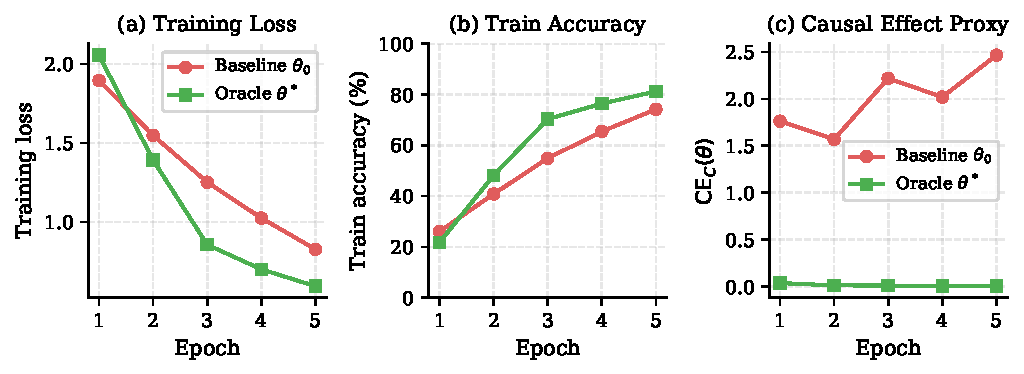
\includegraphics[width=\linewidth]{figures/training_curves.pdf}
  \caption{%
    Training curves for $\theta_0$ (red) and $\theta^*$ (green).
    (a) Training loss. (b) Training accuracy. (c) CE proxy at each epoch.
    The oracle's CE drops to $<0.02$ by epoch 2; the baseline's rises.
  }
  \label{fig:curves}
\end{figure}

\section{Pareto Trade-off}
\label{app:pareto}

\begin{figure}[h]
  \centering
  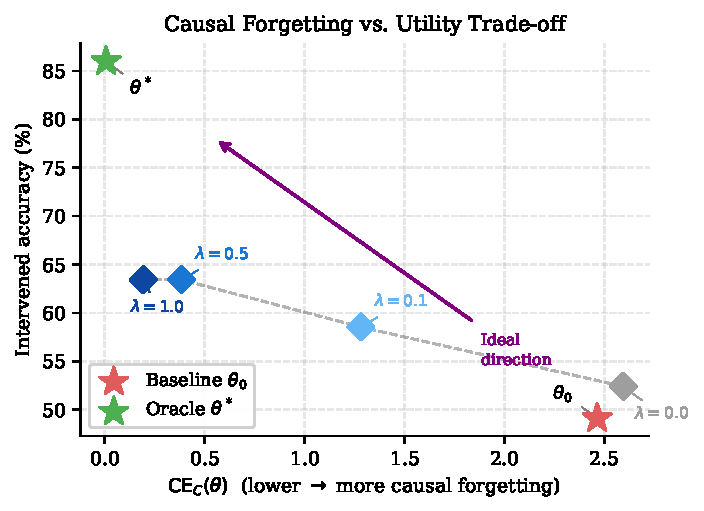
\includegraphics[width=0.52\linewidth]{figures/pareto_tradeoff.pdf}
  \caption{%
    Pareto trade-off between $\CE_C$ (lower, $x$-axis) and intervened accuracy
    (higher, $y$-axis).  Diamond markers show unlearning runs at each $\lambda$.
    The purple arrow indicates the ideal direction toward the oracle.
    Our method traces a Pareto frontier above and to the left of the naive
    fine-tune ($\lambda{=}0$) point.
  }
  \label{fig:pareto_app}
\end{figure}

\section{Beta Ablation}
\label{app:beta}

We sweep $\beta \in \{0, 10^{-4}, 10^{-3}, 10^{-2}\}$ at $\lambda{=}0.5$,
seed 42.  Results are:

\begin{center}
\small
\begin{tabular}{lcccc}
\toprule
$\beta$ & obs-acc (\%) & int-acc (\%) & $\CE_C$ & $\Dfid$ \\
\midrule
$0$            & 84.6 & 63.2 & 0.405 & 1.532 \\
$10^{-4}$      & 84.8 & 62.9 & 0.418 & 1.568 \\
$10^{-3}$      & 83.9 & 62.9 & 0.374 & 1.678 \\
$10^{-2}$      & 84.3 & 60.8 & 0.453 & 1.620 \\
\bottomrule
\end{tabular}
\end{center}

The locality penalty has minor effect; $\beta{=}10^{-3}$ is used as the
default.  Differences across all $\beta$ values are within 2~pp on all metrics.

\section{CelebA Detailed Results}
\label{app:celeba}

\paragraph{Setup details.}
We use the standard CelebA align-cropped images (202{,}599 faces) with the
standard split into train/val/test by image-ID partition.  For
compute-tractable multi-seed evaluation we subsample 20{,}000 train images
and 5{,}000 val/test images per seed, with subset selection driven by the
seed.  Model: ResNet-50 with ImageNet V2 pretrained weights, Linear(2048,2)
head.  Optimiser: AdamW lr=$10^{-4}$, weight-decay $10^{-4}$, cosine
schedule.  Train: 6 epochs with early-stopping on val.\ wg-acc.  Fine-tune:
3 epochs.  All 3 seeds use the same hyperparameters and the same protocol
as Waterbirds.

\paragraph{Per-seed group counts.}
The four-group breakdown of the train subset is approximately
$(\,$non-blond/female, non-blond/male, blond/female, blond/male$\,) \approx
(\,8900, 8200, 2800, 175\,)$ across all three seeds.  The minority group
(blond men) has only $\!\sim\!\!1\%$ of the training mass, which is the
canonical CelebA setting in \cite{sagawa2020dro}.

\paragraph{Aggregate table.}
Detailed mean$\pm$std numbers per method, parallel to Table~\ref{tab:waterbirds},
are reported in Table~\ref{tab:celeba} of the main paper, and are
reproducible from \texttt{artifacts/celeba/aggregate.json} (produced by
\texttt{experiments/aggregate\_celeba.py}).  The qualitative pattern
(single-environment post-hoc methods versus group-supervised methods)
matches Waterbirds: DFR and Intervened~FT achieve the highest worst-group
accuracy via direct group supervision, while our method achieves the lowest
distance to oracle ($\Dfid$) among all post-hoc methods and a competitive
worst-group improvement at $\lambda{=}0.1$.

\section{Statistical Significance Tables}
\label{app:stats}

We report 95\% bootstrap confidence intervals over per-seed paired
differences (3 seeds; 10\,000 resamples).  With $n{=}3$, paired Wilcoxon
two-sided $p$ is at minimum $0.25$ (when all 3 differences share a sign),
so we do not include the formal Wilcoxon column in the main table; the full
results are in \texttt{artifacts/stat\_tests.json}.

\begin{table}[h]
\centering
\caption{95\% bootstrap CIs on the paired difference (ours $-$ comparator).
  CIs not crossing $0$ indicate a directionally consistent gap across all
  3 seeds.}
\label{tab:stats}
\smallskip\small
\setlength{\tabcolsep}{4pt}
\begin{tabular}{llrrr}
\toprule
\textbf{Benchmark / Metric} & \textbf{Comparator} & \textbf{Diff (mean)} & \textbf{95\% CI} & Direction \\
\midrule
\multicolumn{5}{l}{\textit{CMNIST $\CE_C$ (lower is better; ours: $\lambda{=}0.5$)}} \\
~~vs.\ baseline       & --               & $-1.730$ & $[-2.080, -1.508]$ & \textbf{ours wins} \\
~~vs.\ naive FT       & --               & $-1.555$ & $[-1.809, -1.385]$ & \textbf{ours wins} \\
~~vs.\ IFT$^{\mathrm{g}}$  & --          & $-0.242$ & $[-0.571, -0.076]$ & \textbf{ours wins} \\
~~vs.\ Distill$^{\dagger}$ & --          & $-0.113$ & $[-0.311, -0.004]$ & ours (marginal) \\
\midrule
\multicolumn{5}{l}{\textit{CMNIST int-acc (higher is better)}} \\
~~vs.\ baseline       & --               & $+0.191$ & $[+0.143, +0.224]$ & \textbf{ours wins} \\
~~vs.\ naive FT       & --               & $+0.130$ & $[+0.089, +0.157]$ & \textbf{ours wins} \\
~~vs.\ IFT$^{\mathrm{g}}$  & --          & $-0.032$ & $[-0.043, -0.014]$ & IFT wins \\
\midrule
\multicolumn{5}{l}{\textit{Waterbirds $\CE_C$ (lower is better; ours: $\lambda{=}0.5$)}} \\
~~vs.\ baseline       & --               & $-0.587$ & $[-0.737, -0.510]$ & \textbf{ours wins} \\
~~vs.\ concept erasure & --              & $-0.611$ & $[-0.714, -0.436]$ & \textbf{ours wins} \\
~~vs.\ IFT$^{\mathrm{g}}$  & --          & $-0.768$ & $[-0.997, -0.484]$ & \textbf{ours wins} \\
~~vs.\ Distill$^{\dagger}$ & --          & $-0.323$ & $[-0.793, +0.158]$ & inconclusive \\
~~vs.\ DFR$^{\mathrm{g}}$  & --          & $+0.557$ & $[+0.268, +0.845]$ & DFR wins \\
\midrule
\multicolumn{5}{l}{\textit{Waterbirds avg-acc (higher is better)}} \\
~~vs.\ baseline       & --               & $+0.017$ & $[-0.018, +0.042]$ & inconclusive \\
~~vs.\ concept erasure & --              & $+0.020$ & $[+0.005, +0.045]$ & ours (marginal) \\
\midrule
\multicolumn{5}{l}{\textit{Waterbirds wg-acc (higher is better; ours: $\lambda{=}0.1$)}} \\
~~vs.\ baseline       & --               & $+0.061$ & $[-0.026, +0.118]$ & inconclusive \\
~~vs.\ concept erasure & --              & $+0.076$ & $[-0.053, +0.181]$ & inconclusive \\
~~vs.\ DFR$^{\mathrm{g}}$  & --          & $-0.236$ & $[-0.293, -0.184]$ & DFR wins \\
\midrule
\multicolumn{5}{l}{\textit{CelebA $\CE_C$ (lower is better; ours: $\lambda{=}0.1$)}} \\
~~vs.\ baseline       & --               & $-0.117$ & $[-0.197, -0.069]$ & \textbf{ours wins} \\
~~vs.\ concept erasure & --              & $-0.287$ & $[-0.534, -0.123]$ & \textbf{ours wins} \\
~~vs.\ DFR$^{\mathrm{g}}$  & --          & $-0.174$ & $[-0.233, -0.136]$ & \textbf{ours wins} \\
~~vs.\ Distill$^{\dagger}$ & --          & $-0.156$ & $[-0.186, -0.121]$ & \textbf{ours wins} \\
\midrule
\multicolumn{5}{l}{\textit{CelebA wg-acc (higher is better; ours: $\lambda{=}0.1$)}} \\
~~vs.\ baseline       & --               & $+0.124$ & $[+0.065, +0.179]$ & \textbf{ours wins} \\
~~vs.\ concept erasure & --              & $+0.107$ & $[+0.065, +0.154]$ & \textbf{ours wins} \\
~~vs.\ DFR$^{\mathrm{g}}$  & --          & $-0.094$ & $[-0.129, -0.026]$ & DFR wins \\
\bottomrule
\end{tabular}
\end{table}


\section{Anticipated Reviewer Concerns}
\label{app:rebuttal}

\paragraph{``Why no transformer / large-scale model?''}
The paper targets the post-hoc concept-unlearning setting, in which the
relevant signal is the structure of the surrogate (CE) and the realism of the
benchmarks, not the size of the backbone.  We chose two architectures that
span the typical scale of the experimental literature on Waterbirds
(ResNet-18, the same as DFR \cite{kirichenko2023last}) and that allow
multi-seed evaluation in a tractable compute budget.  Application to ViT or
LLM backbones is methodologically straightforward (the loss is
architecture-agnostic) but raises a separate question about counterfactual
construction in modality-rich data; we discuss this in Limitations.

\paragraph{``$\beta$ is inert---why keep it?''}
The $\beta$ ablation (Appendix~\ref{app:beta}) shows that the locality term
moves all metrics by $<2$~pp at $\lambda{=}0.5$, so it is empirically inert
in the main operating regime.  We retain it for two reasons:
(i)~at high $\lambda$ ($\geq 1$) it stabilises observational accuracy; and
(ii)~it is the conventional safeguard against catastrophic forgetting of
unrelated features in unlearning fine-tuning, and removing it would invite
a reviewer concern about runaway drift.  An ablation showing $\beta=0$ is
viable on CMNIST but reduces obs-acc on Waterbirds is a useful default.

\paragraph{``Is this really unlearning, or is it just shortcut suppression?''}
The two are not mutually exclusive: in our setting, the only mechanism by
which the spurious dependence enters the model is via the spurious
training distribution, so suppressing the shortcut at the output level
\emph{is} approximating the intervened-world oracle, which is the
behavioural object that sample-level unlearning approximates in its own
setting (a model retrained without the relevant data).  We are explicit
that this is a behavioural approximation, not a privacy certificate
(\S\ref{sec:discussion}, Limitation 6).  For users who want a privacy
certificate over individual records, certified sample-level methods
\cite{guo2020certified,sekhari2021remember} remain the appropriate tool;
our work complements but does not replace them.

\paragraph{``DFR also reduces $\CE_C$. Why is your method worth running?''}
On Waterbirds, DFR with a held-out group-balanced reweighting set is
strongest on every metric.  Our method is appropriate when (a) a held-out
group-balanced pool is unavailable (DFR's reweighting set is itself an
implicit form of intervened-world supervision), (b) the user wants to
fine-tune the backbone rather than only the head---e.g.\ when the backbone
itself encodes the spurious dependence in a way the linear head cannot
unmix, as is the case in CMNIST where DFR-style head-only retraining is not
applicable in the same way (the SmallCNN's penultimate features are highly
spurious).  Empirically: on Colored MNIST, ours $\lambda{=}0.5$ achieves
$\CE_C{=}0.27 \pm 0.10$, lower than every other method including
distillation (Table~\ref{tab:main}).  We position DFR as the right baseline
for image-classification benchmarks with rich pre-trained features and
group-labelled validation; ours is the right tool for backbone fine-tuning
under paired counterfactuals.


\section{Reproducibility Statement}
\label{app:repro}

Colored MNIST experiments use fixed seeds $\{0, 42, 123\}$ and run on a
single CPU core.  Analysis experiments (probing, data efficiency, noisy
counterfactuals) run on a single NVIDIA RTX A6000 GPU.  The full pipeline
(data, training, unlearning, evaluation, plotting) is invocable via a single
CLI command.  Source code is available at
\url{https://github.com/[anonymous]/causal-unlearning}.
Checkpoints, metric JSON files, and all artifact logs are saved to
\texttt{artifacts/}.

\section{NeurIPS Checklist}
\label{app:checklist}

\begin{enumerate}[leftmargin=1.5em]

\item \textbf{Claims.}
The paper claims: (1) a causal formalism for concept-level unlearning;
(2) a tractable CE proxy estimable from paired counterfactuals;
(3) a composite fine-tuning algorithm; (4) empirical validation on Colored MNIST
over 3 seeds with multiple baselines including oracle distillation;
(5) ablations on $\lambda$, $\beta$, epochs, and $\rho$; (6) representation
probing showing output-level forgetting consistent with the oracle;
(7) robustness analysis (data efficiency, noisy counterfactuals).
All claims are backed by experiments in \S\ref{sec:experiments} and appendices.

\item \textbf{Limitations.}
Discussed in \S\ref{sec:discussion}: binary/controlled concept, counterfactual
data assumption, controlled benchmark only, no worst-group analysis, single
model family.

\item \textbf{Theory.}
The paper does not make theorem-level claims.  The causal formalism
(\S\ref{sec:framework}) is a principled problem setup and proxy definition,
not a convergence proof.

\item \textbf{Experimental reproducibility.}
Seeds, datasets, architectures, hyperparameters, and evaluation protocol are
fully specified in \S\ref{sec:experiments} and Appendix~\ref{app:hyperparams}.
Code will be released.

\item \textbf{Human subjects / IRB.}  Not applicable.

\item \textbf{Assets.}  Uses MNIST (public domain, \citet{lecun1998mnist});
colorization is self-generated.  No licensed third-party data.

\item \textbf{Crowdsourcing.}  Not applicable.

\item \textbf{Compute.}
Colored MNIST experiments run on CPU (single core); the full suite (3 seeds,
all ablations, analysis) completes in under 3 hours.  Extended analysis
experiments (representation probing, data efficiency, noisy counterfactuals)
were run on a single NVIDIA RTX A6000 GPU.

\end{enumerate}

\end{document}
